%\documentclass[a4paper]{memoir}
\documentclass[a4paper, 12pt]{report}
\usepackage[top=2.5cm, bottom=2.5cm, left=2.5cm, right=2.5cm]{geometry}
%\documentclass[a4paper]{article}
\usepackage[utf8]{inputenc}
\usepackage[english]{babel}
\usepackage{hyperref}
\usepackage{minted}
\usepackage{amsmath}
\usepackage{graphicx}
\usepackage{xcolor}
\definecolor{light-gray}{gray}{0.95}
%\definecolor{LightGray}{gray}{0.95}
\usepackage{listings}
\lstset{frame=tb,
  language=C++,
  aboveskip=6mm,
  belowskip=6mm,
  showstringspaces=false,
  columns=flexible,
  basicstyle={\small\ttfamily},
  numbers=none,
  numberstyle=\tiny\color{gray},
  keywordstyle=\color{blue},
  commentstyle=\color{dkgreen},
  stringstyle=\color{mauve},
  breaklines=true,
  breakatwhitespace=true,
  tabsize=3,
  backgroundcolor=\color{light-gray},
  %language=Matlab
}
%\usepackage{color}
\usepackage{float}
\usepackage[justification=centering]{caption}
\usepackage{caption}
\usepackage{verbatim}
\usepackage{xifthen}
\usepackage{tikz}
\usepackage{lscape} 
\usepackage{pdflscape}
\usepackage{diagbox}
\usepackage{multirow}
\usepackage{algorithm}
\usepackage{algorithmic}
\let\oldv\verbatim
\let\oldendv\endverbatim
\usepackage[square,sort,comma,numbers]{natbib}
\usepackage[OLDMEK, 30]{masterfrontpage}
\usepackage[edges]{forest}
\definecolor{folderbg}{RGB}{124,166,198}
\definecolor{folderborder}{RGB}{110,144,169}
\newlength\Size
\setlength\Size{4pt}
\tikzset{%
  folder/.pic={%
    \filldraw [draw=folderborder, top color=folderbg!50, bottom color=folderbg] (-1.05*\Size,0.2\Size+5pt) rectangle ++(.75*\Size,-0.2\Size-5pt);
    \filldraw [draw=folderborder, top color=folderbg!50, bottom color=folderbg] (-1.15*\Size,-\Size) rectangle (1.15*\Size,\Size);
  },
  file/.pic={%
    \filldraw [draw=folderborder, top color=folderbg!5, bottom color=folderbg!10] (-\Size,.4*\Size+5pt) coordinate (a) |- (\Size,-1.2*\Size) coordinate (b) -- ++(0,1.6*\Size) coordinate (c) -- ++(-5pt,5pt) coordinate (d) -- cycle (d) |- (c) ;
  },
}
\usetikzlibrary{calc}
%\usetikzlibrary{decorations.pathmorphing}
\usetikzlibrary{%
    decorations.pathreplacing,%
    decorations.pathmorphing%
}
\forestset{%
  declare autowrapped toks={pic me}{},
  pic dir tree/.style={%
    for tree={%
      folder,
      font=\ttfamily,
      grow'=0,
    },
    before typesetting nodes={%
      for tree={%
        edge label+/.option={pic me},
      },
    },
  },
  pic me set/.code n args=2{%
    \forestset{%
      #1/.style={%
        inner xsep=2\Size,
        pic me={pic {#2}},
      }
    }
  },
  pic me set={directory}{folder},
  pic me set={file}{file},
}

\title{NEED A TITLE!!!}
\author{Peter Even Killingstad}
\pagenumbering{roman} % Start roman numbering
\begin{document}
\masterfrontpage
\begin{abstract}
Computational fluid dynamics, with the software OpenFOAM, has ben used to investigate the dead water phenomenon. Investigation was done by simulating a barge moving in stratified waters. Comparison of the turbulence models $k-\epsilon$ and $k-\omega$ SST has been conducted, resulting in a better performance in estimating drag by the $k-\omega$ SST model. Simulations of the barge moving in stratified fluid is shown to generate internal gravity waves below and in the wake of the barge. The internal gravity waves cause the barge to experience an increase in drag for subcritical densimetric Froude numbers ($Fr_h$). Maximum drag is shown to appear in regions of $0.6 \leq Fr_h \leq 0.7$. Internal gravity waves restrict the passage area causing an acceleration of the flow downstream of the barge, resulting in thinning of boundary layer and in drop of pressure.
\end{abstract}
\chapter*{Acnowledgements}

\tableofcontents

\chapter{Introduction}
\pagenumbering{arabic} % Switch to normal numbers
Dead water is the phenomenon where internal gravity waves are causing boats or vessels moving along the surface of a stratified fluid, to experience increased drag force. A stratified fluid can be observed in the ocean where layers have different salinity, or temperature jumps, causing a difference in density. Rapidly melting glaciers can produce a layer of fresh water on top of denser ocean salt water, or a layer of warmer ocean currents can be lying on top of colder currents. The internal gravity waves occur where the maximum vertical density gradient exist, called the pycnocline.\\
\\
The Norwegian scientist and explorer Fridtjof Nansen was the first to describe the phenomenon \citep{Nansen}. During the FRAM expidition while passing north of Sibira, his boat FRAM experienced a reduction in speed to about a fifth, even though the engine was working on full power. As the speed was reduced, F. Nansen observed internal waves accross the wake, arising sometimes as far as almost midships. Ekman later conducted the first experimental study on the phenomenon\cite{Ekman}, by using a towing tank with stratified water conditions. The study concluded that the model experienced an increase in drag force due to the internal waves.\\
\\
\begin{figure}[H]
	\centering
	\includegraphics[width=0.70\textwidth]{/home/peterek/OpenFOAM/PETER-5.0/MT_PK/plots/paraView/surfaceContour/surfaceCountourIf02U022.png}
	\caption{Internal wave below a barge\\ \textit{Visualization of an internal wave below and in the wake of a barge made by simulating with Computational fluid dynamics. The internal waves occur at the pycnocline located at 0.2 m below the surface.}}
	\label{fig:eta0}
\end{figure}
This project is mainly motivated by the recently published work of J. Grue \cite{Grue}, Gou et al. \cite{Gou} and Esmaeilpour et al. \cite{Esmaeilpour}.\\
J. Grue investigated the dead water resistance on the Polar ship FRAM by using two methods. The first is empirical, using F. Nansens own observations, and the other is a strongly non linear interfacial method in three dimensions.\\
Gou et al. investigated drag force on a barge in two layer fluid. The investigation was done by conducting three dimensional experiments in a towing tank. \\
Esmaeilpour et al. studied dead water resistance on a vessel by simulating the phenomenon using computational fluid dynamics.\\
\\
The Navier-Stokes equation is the fundamental equation describing viscous fliud flow, including the dead water phenomenon. In this project, the dead water phenomenon is studied by using computational fluid dynamics. In order to fully resolve the 3-dimensional Navier-Stokes equation, computer simulation and discretization is needed as no explicit solution exists. Simulations of experiments on a barge moving in stratified water is done by using the free open sorce software OpenFOAM.\\
\\
The main focus of the project is to study the drag force and the increase in drag due to stratified water. Non-stratified and stratified fluid simulations are conducted for qualitative understanding and comparison. Three different pycnocline depths are simulated for the stratified fluid experiments. Simulations are done with different speeds in order to obtain densimetric Froude numbers in regions $0.35 \leq Fr_h \leq 1.35$.\\
\\
Increase in drag is presented for each pycnocline depth. Peak drag is shown to occur within a range of densimetric Froude number of $0.6 < Fr_h < 0.7$. The position of the internal gravity wave and its location below the barge is shown to have significant effect on the drag. Depending on the location of the internal gravity waves, velocity profiles below the stern of the barge are shown to be significantly effected \\
\\
As the barge is moving through the stratified water, the flow is turbulent. To fully obtain details of the rapidly fluctuating flow is impossible, as it reqiures a huge amount of computational power. Various techniques of modelling turbulent flow are presented. This project is using Reynolds avaraged Navier-Stokes (RANS) equations, a method focusing on the mean fliud flow.Two RANS turbulence models are presented, tested and compared to find the most suitable model for simulating dead water.\\
\\
Stratified fluid simulations deal with fresh and salt water with different densities. OpenFOAM has several multi phase solvers implemented. This project is using the solver \textit{twoLiquidMixingFoam} which solves the multi phase problem using the volume of fluid-method, and is applicable for two miscible fluids.\\
\\
OpenFOAM is using the finite volume method, a numerical technique to discretize the equations. Brief motivation for applying the method is presented, along with a differential scheme. A computational domain has been made that consitst of a mesh grid in which the discretized equations can be solved. The computational domain needs to be well defined at the boundaries in order to get meaningfull results. Initial and boundary conditions are defined for all the variables in the equations.\\
\\
Quality of the mesh is essential in order to get reliable results. Convergence tests of three systematically refined grids are conducted to make sure that the mesh used in the simulations are stable, and at the same time is computational efficient.\\
\\
In the following chapters, theory, introduction to OpenFOAM, simulation design, results and finally a conclusion is presented.\\
\\
The first chapter contains introduction to the governing equations of the thesis. It further gives a brief description of physical concepts of turbulence, boundary layer theory and computer modelling of turbulence. The theory behind the volume of fluid-method is presented, and finally an outline of the finite volume-method used to discretize the equations is presented.\\
\\
The following chapter introduces the open software OpenFOAM, and its structure used in the solving procedure.\\
\\
The simulation design chapter describes the numerical experiment, with domain geometry and physical setup. It further presents Initial and boundary conditions before mesh quality and convergence tests are presented.\\
\\
The rusults are shown and discussd. A conclusion is reached and further recomendations are presented.  
\chapter{Theory: Governing equations, Turbulence, and Numerical methods.}
\section{Governing equations}
The study of viscous flow reaches back to acient times. Humans figured out, with clever intuision, trial and error, the importance of viscous friction. Long before any real theoretical understanding of fluid flow, streamlined weapons and boats have been made to overcome the effects of viscosity. In more recent years the understanding has taken huge leaps. Today we have tools to master viscous flow with the help from theory. The fundamental equation describing viscous flow is called Navier-Stokes equation\cite{White}. With the following assumptions: incompressible, newtonian fluids. Density and viscosity may be different, but for one fluid it is constant. This gives the following equations:
\begin{eqnarray}
\label{eqn:continuity}
\nabla \cdot \mathbf{u} &=& 0 \\ 
\label{eqn:momentum}
\frac{\partial \rho \mathbf{u}}{\partial t} + \nabla \cdot \big(\rho \mathbf{u} \mathbf{u}\big) &=& \nabla p + \mu \nabla^2 \mathbf{u} + \rho\mathbf{g} + \mathbf{f}_{st} 
\end{eqnarray}
where (\ref{eqn:continuity}) is the conservation of mass and (\ref{eqn:momentum}) is the conservation of momentum. $\mathbf{u}$ is the velocity, $p$ is the pressure, density is given by $\rho(\mathbf{x},t)$, the dynamic viscosity is given by $\mu$, $\mathbf{g}$ and $\mathbf{f}_{st}$ is the gravity and surface tension respectively. There are four independent variables, the spatial $x, y$ and $z$ coordinates, and the time $t$.\\
\\
The equations are a set of coupled differential equations. In practice, these equations are to difficult to solve analytically, but solutions for some simple geometries and boundary conditions can be found. More complex cases, as almost all flows of engineering significance, needs to bee approximated with numerical techniques. Computational fliud dynamics has become the most viable tool to represent the complex Navier-Stokes equations. Some CFD models will be briefly introduced later in this chapter.\\
\\
Using Navier stokes (\ref{eqn:continuity} and \ref{eqn:momentum}), the goal would be to investigate the forces in most industrial and academic applications. Finding solutions to the equations, either analytical or approximations, makes it possible to calculate the force vector by using:
\begin{equation}
\mathbf{F} = \int_{surface} \Big(\nu\big(\nabla \mathbf{u} + (\nabla \mathbf{u})^T\big) - p \mathbf{I}\Big) \cdot \mathbf{n} ds.
\label{eqn:forceVector}
\end{equation}
$\mathbf{n}$ is the unit vecctor normal to the surface, $\mathbf {I}$ is the unit matrix and $\nu$ is the kinematic viscosity. \\
\\
Having obtained the force vector, it is usual to quantify the the drag force or resistance by introducing the drag coefficient, a dimensionless quantity given by
\begin{equation}
C_d = \frac{F_d}{\frac{1}{2}\rho S u^2}.
\label{eqn:dragCoeff}
\end{equation}
Here $F_d$ is the drag force, $\rho$ is density, $u$ is the freestream velocity and $S$ is the surface area. \\
\\
Viscous flows can be divided into several regimes, and the primary controlling parameter is the dimensionless Reynolds number\cite{White}.
\begin{equation}
Re = \frac{u_0l_0}{\nu}
\label{eqn:ReynoldsNumber}
\end{equation}
where $u$ is a velocity scale, $l_0$ is a characteristic geometric size and $\nu$ is the kinematic viscosity. $Re$ represents the ratio of inertial forces to viscous forces within a fluid flow. Fluid properties can cause dramatic changes to the flow patterns. It is usual to divide flows into three distinct regimes.
\begin{itemize}
	\item Low Re flow: \\ Viscous forces dominates and the flow is smooth or laminar regime.
	\item Intermidieate Re flow: \\ Flow is in a transitional region where it is partly fluctuating and partly laminar regime.
	\item High Re flow: \\ Inertial forces dominates and the flow is fluctuating or in a turbulent regime.
\end{itemize} 
Objects advancing through fluids such as water generate free surface waves. At the same time, if an object is advancing through stratified fluids, it generates internal waves. While free surface waves depend on the Froude number: 
\begin{equation}
Fr = \frac{U_0}{\sqrt{gL_0}},
\label{eqn:FroudeNumber}
\end{equation} 
internal waves depends on the densimetric Froude number:
\begin{equation}
Fr_h = \frac{U_0}{c^*}.
\label{eqn:densimetricFroudeNumber}
\end{equation}
$U_0$ is the ship speed, $g$ is gravity and $L_0$ is the ship length at water level. $c^*$ represents the celerity of the longest internal waves. For an infinitely deep stratified fluid, $c^*$ is given as:
\begin{equation}
c^* = \sqrt{gh\frac{\Delta \rho}{\rho_0}}
\label{eqn:celerityWaves}
\end{equation} 
where h is the distance from the free surface to the pycnocline, $\Delta \rho$ is the difference beetwen the density of the stratified fluid.
\section{Turbulence}
\subsection{Physical concepts of turbulence}
Turbulence is the phenomenon where a fluid flow appears to be chaotic and random. Unlike laminar flow, where the fluid flows in an orderly fashion, turbulent flow is rapidly fluctuating in all spatial dimensions. Structures of the flow is varying from large scales comparable to the dimensions of the physical boundaries to small scales.\\
\\
The main characteristics of turbulence is the transfer of energy from larger spatial scales into smaller, happening in a three dimensional space and time.\\
\\
 To discuss the main characteristics of turbulence, a usefull concept is that of an "eddy". An eddy can be thought of as typical turbulence pattern of small- and large- scales all co-existing in the same fluid. The eddies consists of vortexes intertwined in a chaotic manner, beeing streched by the mean flow and pulled in random directions by one another. This mechanism ultimately leads to braking of the eddies into smaller ones, leading to an "energy cascade"\cite{CFD}.\\
\\
The kinetic energy of the mean flow is extracted by the largest scale eddies. Energy from the largest eddies is further extracted to smaller scales, and the kinetic energy is finally dissipated into thermal energy by the small scale eddies \cite{CFD}.\\
\\
The turbulent kinetic energy is defined by the units $\sim [m^2/s^2] \sim u_0^2$. As turbulence is dissipative, the dissipation rate has the units $[m^2/s^3]$. The dissipation rate of kinetic energy scales as $\epsilon \propto u_0^3/l_0$ \cite{Turbulence}, where $u_0$ and $l_0$ is the characteristic velocity and length of the flow.\\
\\
The dissipation rate of kinetic energy is one of the most important results of turbulence theory, and is reffered to as the Kolmogorov relation \cite{Turbulence}. A turbulent eddy with kinetic energy $u_0^2$ either looses its energy or breaks up into smaller eddies in one time scale or period $T \sim l_0/u_0$.\\
\\

As Reynolds number is very large for turbulent flow, i.e $\frac{u_0l_0}{\nu} \gg 1$, the large scale eddies is independent of the viscosity. To see how viscosity is effecting the turbulent flow, "Kolmogorov micro-scales" can be constructed. Using kinematic viscosity $\nu$ and the dissipation rate $\epsilon$, small scale velocity, length and time can be written out as:
\begin{eqnarray}
\label{eqn:microLength}
\eta &=& \big(\frac{\nu^3}{\epsilon}\big)^{1/4}, \\
\label{eqn:microVelocity}
v &=& \big(\nu\epsilon\big)^{1/4}, \\
\label{eqn:microTime}
\tau &=& \big(\frac{\nu}{\epsilon}\big)^{1/2}, 
\end{eqnarray}  
where  $\eta$ is the micro length-scale, $v$ is the velocity and $\tau$ is the time scale. Reynolds number in the "micro-scale" is given by $\frac{v\eta}{\nu} = 1$, hence the viscosity is of big importance at theese scales. We have that the "micro-scale" eddies is dominated by friction, and small-scale turbulence is almost independent of large scale turbulence for large enough reynolds number.

\subsection{Boundary layer}
Using Reynolds number (\ref{eqn:ReynoldsNumber}) it is easily shown that, for a thin shear layer flow over a flat plate, inertial forces dominate. A Reynolds number based on $U= 1$m$s^{-1}$, $l_0= 0.1$m and $\nu = 10e-6m^2s^{-1}$ would be $Re_{l_0} = 10e5$, and inertial forces are much larger than viscous forces.\\
\\
If Reynolds number is based on a length scale $y$ that is decreasing towards $0$, $Re_y$ would eventually be $\mathcal{O}(1)$. The viscous forces is then either equal or bigger than the inertial forces.\\
\\
This close to the wall, the mean velocity depends on the distance $y$, fluid density $\rho$, viscosity $\nu$ and the wall shear stress $\tau_w$, and is usually called the turbulent boundary layer \cite{CFD}.\\
\\
By using dimensinal analysis, flow behaviur can be expressed by means of dimensionless groups $u^+$ and $y^+$.\\
\\
The dimensionless groups are given by \cite{CFD}
\begin{eqnarray}
\label{eqn:upluss}
u^+ &=& \frac{U}{u_*}\\
\label{eqn:ypluss}
y^+ &=& \frac{y u_*}{\nu}\\
\label{eqn:uStar}
u_* &=& \sqrt{\frac{\tau_w}{\rho}} 
\end{eqnarray}
$u_*$ is the friction velocity.\\
\\
Turbulent boundary layer consists of two regions:
\begin{itemize}
\item Inner region, consists of tre layers:
	\begin{itemize}
	\item where viscous stresses dominates,
	\item where turbulent stresses dominate,
	\item where viscous and turbulent stresses are of similar magnitude.
	\end{itemize}
\item outer region
	\begin{itemize}
	\item inertia dominated flow far from the wall.
	\end{itemize}
\end{itemize}
The layer where viscous stresses dominates is called the viscous sub-layer. It is a linear relationship between the velocity and distance to the wall and is given as \cite{CFD}
\begin{equation}
u^+ = y^+
\label{eqn:viscousSublayer}
\end{equation}
The layer is extremely thin, and lies at $y^+ < 5$ \cite{CFD}.\\
\\ 
At the layer where turbulent stresses dominates, called the log-layer, the velocity and distance to the wall has a logarithmic relationship. It is given as \cite{CFD}
\begin{equation}
u^+ = \frac{1}{\kappa}\ln(y^+) + B
\label{eqn:logLayer}
\end{equation}
The constants $\kappa = 0.41$  and $B= 5.5$ is found by doing measurements. The log-layer lies outside the viscous sub-layer, at $30 < y^+ < 300$ \cite{CFD}.\\
\\
Between the viscous sub-layer and the log-layer lies the buffer layer, where the viscous and turbulent stresses are of similar magnitude.\\
\\
Equations for the viscous sub-layer and log-layer (\ref{eqn:viscousSublayer} and  \ref{eqn:logLayer}) are usually called law of the wall and are of great importance in approximating and simulating turbulent boundary layers.\\
\\
Figure \ref{fig:lawOfTheWall} is showing a plot containing the viscous sub-layer and the log-layer
\begin{figure}[H]
	\centering
	\includegraphics[width=0.70\textwidth]{/home/peterek/OpenFOAM/PETER-5.0/MT_PK/plots/turbulenceModelComparison/lawOfTheWall.png}
	\caption{Law of the wall\\ \textit{law of the wall; Viscous sub-layer in blue in the range $y^+ < 5$ and log-layer given in green in the range $30 \leq y^+ \leq 300$. Inbetween the viscous sub-layer and log-layer lies the buffer layer. Outer region lies where $y^+ > 300$}}
	\label{fig:lawOfTheWall}
\end{figure}

 
\subsection{Computer modelling of turbulence}
The modelling of turbulent fluid flows and the Navier-Stokes equations has seen huge advancements as computer speed increases. The number of applications of fluid flow predictions has grown and computerized analysis has become a crucial part in the field of fliud mechanics.\\
\\
There are three main methods for numerically solving Navier-Stokes equations:
\begin{itemize}
	\item Reynolds Averaged Navier Stokes(RANS)
	\item  Large Eddy Simulations(LES)
	\item  Direct Numerical Simulations(DNS)
\end{itemize}
LES and DNS is introduced rather briefly, while RANS will be introduced in a litle bit more detail.
\subsubsection{RANS}
For many enginering purposes, the focus is on the mean effect of turbulence, and it is unecessary to resolve the details on all scales.\\
\\
A key part of RANS is investigating the effects of fluctuations on the mean flow using Reynolds de-composition. The velocity and pressure is decomposed as:
\begin{eqnarray}
\label{eqn:ReynoldsDecompU}
\mathbf{u} &=& \mathbf{U} + \mathbf{u'} \\
\label{eqn:ReynoldsDecompP}
p &=& P + p',
\end{eqnarray}
where $\mathbf{u}$ is the instantaneous flow field, $\mathbf{U}$ is the mean flow field and $\mathbf{u'}$ is the fluctuating part. The same goes for the pressure, where P is mean and p' is the fluctuating part.\\
\\
Substituting the de-composed velocity and pressure (\ref{eqn:ReynoldsDecompU}, \ref{eqn:ReynoldsDecompP}) into Navier-Stokes equations (\ref{eqn:continuity}, \ref{eqn:momentum}) and taking the time-mean, the following continuity and momentum equations using suffix notation is derived:
\begin{eqnarray}
\label{eqn:RANScontinuity}
\frac{\partial U_i}{\partial x_j}  &=& 0 \\
\label{eqn:RANSmomentum}
\frac{\partial U_i}{\partial t} +  \frac{\partial}{\partial x_j}(U_i U_j) &=& -\frac{1}{\rho} \frac{\partial P}{\partial x_i} + \nu \frac{\partial ^2 U_i}{\partial x_j \partial x_j} - \frac{\partial}{\partial x_j} (\overline {u_i' u_j'}).
\end{eqnarray}
Here $U_i$ is the mean velocity, P is the mean pressure and $\overline{u_i'}$ is the mean fluctuating velocity.\\
\\
In the momentum equation (\ref{eqn:RANSmomentum}), the new term $\frac{\partial }{\partial x_j}(\overline{u_i'u_j'})$ is derivative of the Reynolds stress-tensor \citep{UNIK4900}. It appears from the convective part $ \mathbf{u} \cdot \nabla \mathbf{u}$ of Navier-Stokes equations (\ref{eqn:momentum}), and is not really stresses. The physical meaning of the term is the averaged effect of turbulent advection on the mean flow field \cite{UNIK4900}.\\
\\
With the new term, the RANS equations is unclosed, with 6 more unknowns appearing from the Reynolds stress-tensor. The four equations has in total 10 unknowns (pressure, three velocity components and six "stresses"). In order to close the problem, enough equations must be found to solve for all the unknowns. In many models, such as one-equation and two-equation models (see \citep{Wilcox} chapter 4), the Boussinesq eddy-viscosity approximation \citep{CFD} is assumed to be valid. The Reynolds stresses are modelled as follows:
\begin{eqnarray}
\label{eqn:bossinesq}
\tau_{ij} = \overline{u_i'u_j'} = \frac{2}{3}k\delta_{ij} - \nu_t\big(\frac{\partial U_i}{\partial x_j} + \frac{\partial U_j}{\partial x_i}\big)\\
\label{eqn:TurbKineticEnergy}
k = \frac{1}{2}\overline{u_i' u_i'} = \frac{1}{2}\big(\overline{u_1^{'2}} + \overline{u_2^{'2}} + \overline{u_3^{'2}} \big)
\end{eqnarray}
where $k$ is the turbulent kinetic energy per unit mass, $\nu_t$ is the turbulent or eddy viscosity and $\delta_{ij}$ is the Kronecker  delta.\\
\\
Substituting the Boussinesq eddy-viscosity approximation (\ref{eqn:bossinesq}) into the RANS momentum equation (\ref{eqn:RANSmomentum}) leads to:
\begin{equation}
\frac{\partial U_i}{\partial t} +  \frac{\partial}{\partial x_j}(U_i U_j) = -\frac{1}{\rho} \frac{\partial P'}{\partial x_i} +  \frac{\partial}{\partial x_j}\Big[ \big(\nu + \nu_t\big) \frac{\partial U_i}{\partial x_j}\Big].
\end{equation}
where $P' = \big(P + \frac{2k}{3}\delta_{ij} \big)$ called the modified pressure\cite{Pope}, often used in CFD.\\
\\
To complete the closure of the RANS equations, the eddy viscosity term $\nu_t$ needs to be modelled. Dimensional analysis dictates that $\nu_t$ needs to be proportinal to the product of a characteristic velocity and a characteristic length scale \cite{Wilcox,AppliedMathematicalModelling}\\
\\
This paper is using two turbulence models for comparison, namely the two-equation models k-$\epsilon$ and the shear stress transport model $k-\omega$ SST.
\subsubsection{$\boldsymbol{k}-\boldsymbol{\epsilon}$ model}
The standard $k-\epsilon$ model equations is found in a lot of litterature such as \cite{CFD} and \cite{UNIK4900}.\\
\\
The $k-\epsilon$ model is perhaps the most widely used, giving good results in classical shear flows. It does however have shortcomings in accurately predicting adverse pressure gradients and boundary layers. despite its shortcomings, the model is recommended in cases with multiphase problems by som literature, i.e \cite{AppliedMathematicalModelling}.\\
\\ 
The model equations are specified as follows:\\
\\
Kinematic eddy viscosity equation:
\begin{equation}
\mu_t = \rho C_{\mu}\frac{k^2}{\epsilon}
\label{eqn:nutKEpsilon}
\end{equation}
Turbulent kinetic energy equation:
\begin{equation}
\frac{\partial \rho k}{\partial t} + U_j \frac{\partial \rho k}{\partial x_j} = \frac{\partial}{\partial x_j}\Big[\frac{\big( \mu + \mu_t\big)}{\sigma_k}\frac{\partial k}{\partial x_j}\Big] - \rho \epsilon + \rho\tau_{ij}\frac{\partial U_i}{\partial x_j}
\label{eqn:kInKEpsilon}
\end{equation}
Turbulence dissipation rate equation:
\begin{equation}
\frac{\partial \rho \epsilon }{\partial t} + U_j\frac{\partial \rho \epsilon}{\partial x_j} =\frac{\partial }{\partial x_j}\Big[\frac{\big(\mu + \mu_t\big)}{\sigma_{\epsilon}}\frac{\partial \epsilon}{\partial x_j} \Big]  + \rho C_{\epsilon 1}\frac{\epsilon}{k}\tau_{ij}\frac{\partial U_i}{\partial x_j} - \rho C_{\epsilon 2} \frac{\epsilon ^2}{k}
\label{eqn:epsilonInKEpsilon}
\end{equation}
The model equations use the Boussinesq assumption given in equation (\ref{eqn:bossinesq}) and contains five adjustable constants: $C_{\mu}=0.09$, $\sigma_k=1.0$, $\sigma_{\epsilon}= 1.3$, $C_{\epsilon 1}=1.44$ and $C_{\epsilon 2}=1.92$
\subsubsection{$\boldsymbol{k}-\boldsymbol{\omega}$ SST}
$k-\omega$ model is made by Menter \cite{SST} and is found in littarture and such as \cite{CFD} and \cite{Wilcox}.\\
\\
The $k-\omega$ SST turbulence model is a more advanced model which combines $k-\epsilon$ and $k-\omega$ models. The $k-\epsilon$ model has its shortcomings, as stated above. The $k-\omega$ model was made to better predict adverse pressure gradients and boundary layers, but preformed poorer at free streams. Menter \cite{reviewOfSSTModel} proposed a new model which combined the $k-\epsilon$ and the $k-\omega$ models. In litterature like \cite{CFD} it is stated that $k-\omega$ SST model is superior in approximating adverse pressure gradients and boundary layers.\\
\\
Turbulence resources such as \cite{NASA_SST} gives thurough desrcription of the model equations. The two-equation model is specified as follows:\\
\\
Kinematic eddy viscosity equation:
\begin{equation}
\mu_t = \frac{\rho a_1 k}{max\big(a_1\omega, \Omega F_2\big)}
\label{eqn:kOmegaSSTTurbulentViscosity}
\end{equation}
Turbulent kinetic energy equation:
\begin{equation}
\frac{\partial \rho k}{\partial t} + U_j \frac{\partial \rho k}{\partial x_j} = \frac{\partial }{\partial x_j}\Big[\big(\mu + \sigma_k\mu_t\big)\frac{\partial k}{\partial x_j} \Big] + \rho P - \beta^* \rho \omega k
\label{eqn:kOmegaSSTKequation}
\end{equation}
Turbulent specific dissipation rate equation:
\begin{equation}
\frac{\partial \rho \omega}{\partial t} + U_j \frac{\partial \rho \omega}{\partial x_j} =
\frac{\partial }{\partial x_j}\Big[\big(\mu + \sigma_{\omega}\mu_t\big)\frac{\partial k}{\partial x_j} \Big] + \frac{\gamma}{\nu_t} \rho P - \beta \rho \omega^2 + 2\big(1 -F_1\big)\frac{\rho \sigma_{\omega 2}}{\omega}\frac{\partial k}{\partial x_j}\frac{\partial \omega}{\partial x_j}
\label{eqn:kOmegaSSTOmegaequation}
\end{equation}
Here $P = \tau_{ij}\frac{\partial U_i}{\partial x_j}$, and $\tau_{ij}$ is the Boussinesq assumption (\ref{eqn:bossinesq}).
\subsubsection{LES}
While RANS has the main focus on the mean flow, LES is resolving large scale turbulence. While the effects of large eddies on the flow is resolved, the effect of the small scale eddies is included by a sub-grid scale models \cite{CFD}. \\
\\
In LES modeling, a spatial filter is used to separate small sclaes from large scales. The method is started off with a filtering function and a "cutoff" witdh, where all scales greater than the "cutoff" width is resolved. \\
\\
A filtering operation  of the filter function function is done in the following manner \cite{CFD}:
\begin{equation}
\overline{\phi}(\mathbf{x}, t) = \int_{-\infty}^{\infty}\int_{-\infty}^{\infty}\int_{-\infty}^{\infty} G(\mathbf{x}, \mathbf{x'} \Delta)\phi(\mathbf{x'},t)dx_1'dx_2'dx_3',
\label{eqn:filteringOperation}
\end{equation}
where $G(\mathbf{x}, \mathbf{x'} \Delta)$ is the filtering function, $\overline{\phi}(\mathbf{x}, t)$ is the filtered function, $\phi(\mathbf{x'},t)$ is the original unfiltered function and $\Delta$ is the "cutoff" witdh. The overbar indicates spatial filtering and not time averaging as with RANS.\\
\\
Filtering the Navier-stokes equations (\ref{eqn:continuity} and \ref{eqn:momentum}) gives the LES continuity and momentum equations as follows:
\begin{eqnarray}
\label{eqn:LEScontinuity}
\frac{\partial \overline{u}_i}{\partial x_j} &=&0\\
\label{eqn:LESmomentum}
\frac{\partial \overline{u}_i}{\partial t} +  \frac{\partial \overline{u}_i \overline{u}_j}{\partial x_j} &=& -\frac{1}{\rho} \frac{\partial \overline{p}}{\partial x_i} + \nu \frac{\partial ^2 \overline{u}_i}{\partial x_j \partial x_j} - \frac{\partial \tau_{ij}}{\partial x_j}.
\end{eqnarray}
Here the overline denotes filtered flow variable, and $\tau_{ij}$ is the sub-grid scale stresses. The sub-grid scale stresses are part of the unresolved sub-grid scales. \\
\\
For further introduction of the LES model, Books such as \cite{CFD} and \cite{LESTurbulence} and papers such as \cite{AppliedMathematicalModelling} is recomended. 
\subsubsection{DNS}
DNS involves numerical solution of the full Navier-Stokes equations. The method resolves all scales, including the kolmogorov scales (\ref{eqn:microLength}, \ref{eqn:microTime} and \ref{eqn:microVelocity}). It takes the closed form of the four equations and four unknowns and solves it on a sufficiently fine mesh and small enough time step. For flows with small enough Reynolds number (\ref{eqn:ReynoldsNumber}), DNS can serve as a benchmark for the other turbulence models \citep{AppliedMathematicalModelling}.\\
\\
Using "Kolmogorov's micro- scales" (\ref{eqn:microLength} and \ref{eqn:microTime}), ratio's of the largest and smallest scales can be obtained. The ratio of the largest and the smallest scales are proportional to  $Re^{3/4}$ and the ratio of the largest and smallest time scale is proportional to $Re^{1/2}$. $Re = 10^4$ requires a spatial resolution of $\mathcal{O}(10^3)$ in each direction, and the simulation must run for atleast $100$ time steps. Computing meshes with $10^9$ grid points with $100$ time steps is very demanding, even with a modest Reynolds number. Computing industrial flows with higher Reynolds number is impossible with current technology \cite{CFD, AppliedMathematicalModelling}.

\section{Volume of fluid}
When there is multiple fluids in a computation, there is need for an interface tracking or interface capturing. To handle multiple-fluid interactions, the volume of fluid method used.\\
\\
For each fluid component, a volume fraction is introduced. If $V$ is a volume of a cell in a computaional domain, and $\alpha(\mathbf{x}, t)$ is the volume fraction, the volume fraction for two fluids is defined as \citep{VOF2}
\begin{equation}
\alpha(\mathbf{x},t) = \left\{
        \begin{array}{ll}
            1, & \quad \mathbf{x} \in \Omega_l \\
            0, & \quad else
        \end{array}
    \right.
\label{eqn:volumeFraction}    
\end{equation}
where $\Omega_l$ is the part of the domain covered by one fliud $l$.\\
\\
On each grid cell, the integral of the color function is approximated. The discrete volume fraction is written as \citep{VOF2}
\begin{equation}
\alpha_i = \frac{1}{V} \int_{V} \alpha(\mathbf{x},t) dV
\end{equation}
where the subscript $i$ denotes the $i$'th fluid in a system.\\
\\
For miscible fluids the volume fractions are governed by the advection-diffusion equation given as \citep{VOF1}
\begin{equation}
\frac{\partial \alpha_i}{\partial t} + \nabla \cdot (\alpha \mathbf{u}) = D_{ab}\nabla^2 \alpha,
\label{eqn:alphadiffusionEquation}
\end{equation} 
Where $D_{ab}$ denotes diffusivity between miscible fluids. The following constraint must be satisfied due to mass conservation:
\begin{equation}
\Sigma_{i=1}^n \alpha_i= 1
\label{eqn:alphaConstraint} 
\end{equation}
Desity and viscosity are defined as:
\begin{eqnarray}
\label{eqn:alphaRhodiffusion}
\rho = \Sigma_i \rho_i \alpha_i \\
\label{eqn:alphaMudiffusion}
\mu = \Sigma_i \mu_i \alpha_i
\end{eqnarray}

\section{Numerical discretization}
\label{sec:NumericalDiscretization}
Numerical discretization is the prosses of transferring differential equations, such as the Navier- Stokes equations (\ref{eqn:continuity} and \ref{eqn:momentum}), into descrete counterparts.
A discretization method is needed in order to evaluate the equations on computers. \\
\\
There are three discretisation methods generally used when approximating equations. Finite difference method, finite element method and finite volume method.\\
\\
As in most commercial well-established CFD codes, this thesis is using the finite volume method. Fvm is one of the most versitaile discretization techniques used in cfd \cite{CFD}.\\
\\
An outline for the disctretization procedure can be presented with the following steps:
\begin{itemize}
\item Integration of the governing equations of fluid flow all over the finite control volumes of the domain.
\item Conversion of the resulting integral equations into a system of algebraic equations.
\end{itemize}
A steady one convection-diffusion equation of a property $\phi$ without a source term is given as:
\begin{equation}
\nabla \cdot (\rho \mathbf{u} \phi) =  \nabla \cdot (\Gamma \nabla \phi),
\label{eqn:stdConvDiff}
\end{equation}
where $\rho$ is the density, $\mathbf{u}$ is a known velocity and $\Gamma$ is diffusivity.\\
\\
Integrating convection-diffusion equation (\ref{eqn:stdConvDiff}) over a control volume (CV) gives:
\begin{eqnarray}
\int_{CV} \nabla \cdot (\rho \mathbf{u} \phi) dV &=& \int_{CV} \nabla \cdot (\Gamma \nabla  \phi) dV \nonumber \\
\label{eqn:intStdConvDiff}
\Rightarrow \int_{A} \mathbf{n} \cdot (\rho \mathbf{u} \phi) dA &=& \int_{A} \mathbf{n} \cdot (\Gamma \nabla  \phi) dA.
\end{eqnarray}
Gauss integration, i.e. Gauss theorem \cite{CFD} is applied to change the integration over a control volume to an integration over an area.
\begin{figure}[H]
\centering
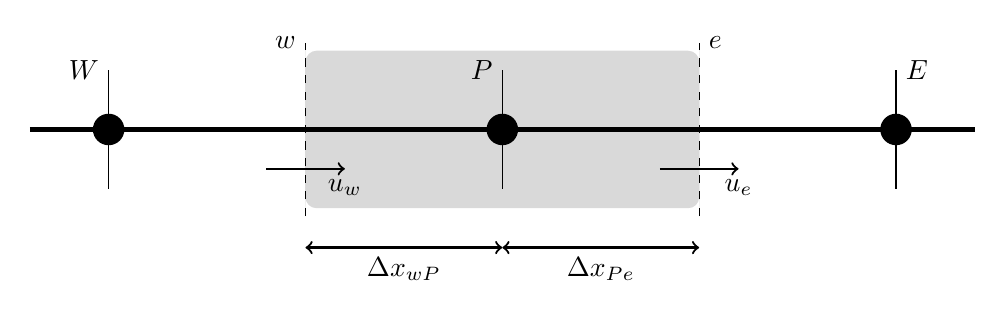
\begin{tikzpicture}
    media/.style={font={\footnotesize\sffamily}},
    wave/.style={
        decorate,decoration={snake,post length=1.4mm,amplitude=2mm,
        segment length=2mm},thick},
    interface/.style={
        % The border decoration is a path replacing decorator. 
        % For the interface style we want to draw the original path.
        % The postaction option is therefore used to ensure that the
        % border decoration is drawn *after* the original path.
        postaction={draw,decorate,decoration={border,angle=-45,
                    amplitude=0.3cm,segment length=2mm}}},
    dimen/.style={<->,>=latex,thin,
        every rectangle node/.style={fill=white,midway,font=\sffamily}},
    ]
	\fill[gray!30,rounded corners] (-2.5,-1) rectangle (2.5,1);	
	\draw[ultra thick,black] (-6,0) -- (6,0);
	%\fill[gray!10,rounded corners] (4,0) rectangle (8,0);
	\fill (-5,0) circle (.2);
	\fill (5,0) circle (.2);
	\fill (0,0) circle (.2);
	\draw[black] (-5,-0.75) -- (-5,0.75) node [left] {$W$};
	\draw[black] (5,-0.75) -- (5,0.75) node [right] {$E$};
	\draw[black] (0,-0.75) -- (0,0.75)node [left] {$P$};
	\draw [fill=gray,dashed] (-2.5, -1.1) --(-2.5, 1.1) node [left] {$w$};
	\draw [fill=gray,dashed] (2.5, -1.1) --(2.5, 1.1) node [right] {$e$};
	\draw[<->,thick] (-2.5,-1.5) -- (0,-1.5) node [midway, below] {$\Delta x_{wP}$};
	\draw[<->,thick] (0,-1.5) -- (2.5,-1.5) node [midway, below] {$\Delta x_{Pe}$};
	\draw[->, thick] (-3,-.5) -- (-2,-.5)node [below] {$u_w$};
	\draw[->, thick] (2,-.5) -- (3,-.5)node [below] {$u_e$};
\end{tikzpicture}
\caption{Control Volume around a cell center P}
\label{fig:ControlVolume}
\end{figure}
In one dimension and using the control volume shown in figure \ref{fig:ControlVolume} the integration of the convection-diffusion equation (\ref{eqn:intStdConvDiff}) gives:
\begin{equation}
\big(\rho u A \phi\big)_e - \big(\rho u A \phi\big)_w = \Big(\Gamma A \frac{d \phi}{dx}\Big)_e - \Big(\Gamma A \frac{d \phi}{dx}\Big)_w.
\label{eqn:intStdConvDiffDiscr} 
\end{equation}
In order to convert the resulting equation (\ref{eqn:intStdConvDiffDiscr}) into a system of algebraic equation, differencing schemes is used.\\
\\
Using central differencing on $d\phi /dx$ at the faces e and w and rewriting the property $\phi$ at the same faces as:
\begin{eqnarray}
\label{eqn:central1}
\phi_w = \frac{\phi_W + \phi_P}{2} \\ 
\label{eqn:central2}
\phi_e = \frac{\phi_P + \phi_E}{2} 
\end{eqnarray}
Substitution of (\ref{eqn:central1}) and (\ref{eqn:central2}) into the resulting equation (\ref{eqn:intStdConvDiffDiscr}) yields the central difference expression:
\begin{equation}
\frac{\rho u_e A_e}{2} (\phi_P + \phi_E) - \frac{\rho u_w A_w}{2} (\phi_W + \phi_P) = \Gamma A_e \frac{(\phi_E - \phi_P)}{\Delta x_{PE}} - \Gamma A_w \frac{(\phi_P - \phi_W)}{\Delta x_{WP}}
\label{eqn:centralDiscretized}
\end{equation}
Rewriting the central difference expression (\ref{eqn:centralDiscretized}), and solving for  $\phi_P$ gives:
\begin{eqnarray}
\Big[(\frac{\rho u_e}{2} - \frac{\Gamma}{\Delta x_{PE}} )A_e  - (\frac{\rho u_w}{2} - \frac{\Gamma}{\Delta x_{WP}} )A_w \Big]\phi_P = \nonumber \\ 
\Big[(- \frac{\rho u_e}{2} + \frac{\Gamma}{\Delta x_{PE}})A_e\Big]\phi_E + \Big(\frac{\rho u_w}{2} + \frac{\Gamma}{\Delta x_{WP}} )A_w \Big]\phi_W
\label{eqn:centralDiscretized2}
\end{eqnarray}
If it is well defined by boundary conditions, the above equation (\ref{eqn:centralDiscretized2}) can be solved as a system of linear equation i.e.:
\begin{equation}
\mathbf{A}\mathbf{x}=\mathbf{b}
\label{eqn:sysOfLinearEqn}
\end{equation}
Where $\mathbf{A}$ is a $m \times n$ matrix, $\mathbf{x}$ is a column vector with $n$ entries and b is a column vector with $m$ entries.\\
\\
Using the FVM, the discretizations is carried directly in the physical domain. There is no need for any transformation between the physical and computational coordinate, making the FVM flexible and popular method for computational fluid dynamics \cite{CFDOpenFOAM}.
\chapter{OpenFOAM}
All computanial fluid dynamis is structured around numerical algorithms that tackles fliud flow problems. Classical solvers are implemented in well-established CFD codes such as CFX/ANSYS, FLUENT and OpenFOAM. The software used in this thesis is OpenFOAM.\\
\\   
As in all well-established CFD codes, the work flow consists of three main elements:
\begin{itemize}
\item pre-processor
\item solver
\item post-processor
\end{itemize}
Pre-processing consists of input of a flow problem, in order to make it well-defined before the solving process begins.\\
\\
The solver is solving the flow problem, by implemented numerical methods and algorithms suitable for the specific problem. \\
\\
Post-processing consists of verification and validation of the solutions given by the solver. It essential to investigate data output and visualize. The complexity of fluid flows demands thurough investigation by e.g. comparing with existing experiments, either numerical or experimental.\\
\\
\section{Introduction to OpenFoam}
\label{sec:IntroductionToOpenFOAM}
This paper is using the free, open sorce software OpenFOAM (Field Operation and Manipulation). It is a C$++$ library of source code for solvers and utilities.\\
\\
Figure \ref{fig:caseStructure} illustrates an initial state of an OpenFOAM case. Three directories are located in the case folder: 0, constant and system.\\
\\
The 0 directory contains files for the different parameters essential for the problem. Each file defines initial values and boundary conditions for the numerical experiment.\\
\\
The \textit{constant} directory contains, as the name suggests, all the constants of the case. Constant variables such as gravitation \textit{g}, \textit{transportProperties} as density and viscosity and \textit{turbulenceProperties} are defined in separate files. The subdirectory \textit{polyMesh} contains the mesh geometry.\\
\\
The \textit{system} directory contains information about meshing of the numerical experiment, how to discretize and solve the equations. The file controlDict controls ehich solver is used, timecontrols and data output controls. As the names suggests, \textit{fvSchemes} and \textit{fvSolution} contains information about discretization schemes and solution algorithms respectively. 
\begin{figure}[H]
\centering
\begin{forest}
  pic dir tree,
  where level=0{}{% folder icons by default; override using file for file icons
    directory,
  },
  [caseDir
    [0
      [u, file]
      [p\_rgh, file]
      [k, file]
      [nut, file]
      [omega, file]
      [alpha.water, file]
    ]
    [constant
      [polyMesh]
      [g, file]
      [transportProperties, file]
      [turbulenceProperties, file]
    ]
    [system
      [blockMeshDict, file]
      [controlDict, file]
      [fvSchemes, file]
      [fvSolution, file]
      [setFields, file]
    ]
  ]
\end{forest}
  \caption{Example of case directory structure in openFOAM.}
  \label{fig:caseStructure}
\end{figure}

\section{TwoLiquidMixingFoam}
\label{sec:TwoLiquidMixingFoam}
OpenFOAM has solvers for a wide range of applications. As mentioned in the section Introduction to OpenFOAM (\ref{sec:IntroductionToOpenFOAM}), the file \textit{controlDict} found in figure \ref{fig:caseStructure} defines which solver to use.\\
\\
Many multiphase solvers can be found, both miscible and immiscible. This thesis is using the incompressible multiphase solver twoLiquidMixingFoam, where the liquids are miscible.\\
\\
Three equations are beeing solved. The first equation is the alpha diffusion equation, given by \cite{Krpan}
\begin{equation}
\frac{\partial \alpha_1}{\partial t} + \nabla \cdot (\mathbf{U} \alpha_1) = \nabla \cdot \Big(\big(D_{ab} + \frac{\nu_t}{S_C}  \big)\nabla \alpha_1 \Big) 
\label{eqn:alphaEqTLMF}
\end{equation}
where
\begin{itemize}
	\item $\alpha_1$ is the volume fraction.
	\item $\alpha_2 = 1 - \alpha_1$	
	\item $\rho = \alpha_1 \rho_1 + \alpha_2 \rho_2 = \alpha_1\rho_1 + (1 - \alpha_1)\rho_2$.
	\item $D_{ab}$ is the molecular diffusivity.
	\item $\nu_t$ is the turbulent eddy viscosity.
	\item $s_c$ is the Schmidt number, given as $\mu / (\rho D)$.
\end{itemize}
The continuity and momentum equation is given, respectively, as: 
\begin{eqnarray}
\label{eqn:continuityTLMF}
\nabla \cdot \mathbf{U} &=& 0 \\
\label{eqn:momentumTLMF}
\frac{\partial \rho \mathbf{U}}{\partial t} + \nabla \cdot(\rho \mathbf{U} \mathbf{U}) &=& - \nabla (p_{rgh}) - gh\nabla \rho + \nabla \cdot (\rho \boldsymbol{\tau})
\end{eqnarray}
where 
\begin{itemize}
	\item $\boldsymbol{\tau} = -\frac{2}{3}\overline{\mu_{eff}}\nabla \cdot \mathbf{U} \mathbf{I} + \overline{\mu_{eff}}\nabla \mathbf{U} + \overline{\mu_{eff}}\big(\nabla \mathbf{U}\big)^T$.
	\item $\overline{\mu_{eff}} = \alpha_1 (\mu_{eff})_1 + \alpha_2 (\mu_{eff})_2$.
	\item $(\mu_{eff})_i = (\mu - \mu_t)_i$. Subscript $i$ denotes either fluid 1 or 2.
\end{itemize}
The term $\nabla(p_{rgh})$ and $gh \nabla \rho$ is obtained by using $P = p_{rgh} + \rho gh$. The Solver is using the Boussinesq eddy-viscosity approximation (\
ref{eqn:bossinesq}), and $p$ is the modified pressure and containes the kinetic energy per unit mass $\frac{2}{3}k\delta_{ij}$.
\section{Turbulence models}
This paper is using the RANS method to approximate turbulence. In order to close the RANS equations, turbulence models are beeing used. Two different two-equation models are implemented for comparison.\\
\\
The turbulence models used in this paper are the $k-\omega$ SST and the $k-\epsilon$ turbulence model. In section Introduction to openFOAM \ref{sec:IntroductionToOpenFOAM}, the \textit{constant} directory shown in figure \ref{fig:caseStructure} contains the file \textit{turbulenceProperties}. Here it is defined what simulation type that is beeing used, i.e. RANS. It also specifies which turbulence model to use.
\section{Numerical schemes}
Having defined the equations to be solved in in section \textit{TwoLiquidMixingFoam} (\ref{sec:TwoLiquidMixingFoam}), the way in which to discretize the equations are defined in the file \textit{fvSchemes} found in figure \ref{fig:caseStructure}. The file consists of sub-dictionaries with name corresponding to terms within the equations given in section \textit{TwoLiquidMixingFoam} (\ref{sec:TwoLiquidMixingFoam}). For each term a numerical scheme must be specified.\\
\\
Time derivative term $\partial / \partial t$ are discretized by using an \textit{Euler} scheme, a first order implicit difference scheme and is given in the sub-dictionary \textit{ddtSchemes}.\\
\\
The other terms are discretized using finite volume method. As explained in section \textit{Numerical discretization} \ref{sec:NumericalDiscretization}, the fvm discretization procedure is done by using gaussian integration and converting the resulting terms into algebraic equations using differencing schemes.\\
\\
Gradient terms $\nabla$ is set in the sub-dictionary \textit{gradSchemes}. The terms are discretized by using \textit{Gauss linear}, where the \textit{Gauss} entry denotes Gaussian integrationand the \textit{linear} entry denotes a central differencing scheme.\\
\\
Divergence terms $\nabla \cdot$ is set in the sub-dictionary \textit{divSchemes}. There are several divergence terms needing discretization, and specified as:
\begin{itemize}
\item \textit{div(rhoPhi,U) Gauss linearUpwind grad(U)}
\item \textit{div(phi,alpha) Gauss vanLeer}
\item \textit{div(phirb,alpha) Gauss linear}
\item \textit{div(phi,k) Gauss upwind}
\item \textit{div(phi,omega) Gauss upwind}
\item \textit{div(((rho*nuEff)*dev2(T(grad(U))))) Gauss linear}
\end{itemize}
The \textit{phi} entry in the \textit{div(phi,...)} is the volumetric flux of velocity. Gauss entry is the Gaussian integration and last entry is the differencing scheme.\\
\\
Laplacian terms $\nabla^2$ is set in the sub-dictionary \textit{laplacianSchemes}, and is discretized as \textit{Gauss linear} with the Gaussian integration and a linear differencing scheme.
\section{Solution algorithms}
There are several solution algorithms implemented in openFOAM. Solution procedures are needed in order to obtain solutions to pressure and momentum. In multiphase modelling, additional solution procedures are needed in order to obtain solution to the phase fraction and the volume of fluid method.\\
\\
There is three different algorithms implemented in OpenFOAM for solving the Navier-Stokes equations (\ref{eqn:momentum}) and (\ref{eqn:continuity}):
\begin{itemize}
\item Semi-implicit method for pressure-linked equations SIMPLE algorithm.
\item pressure-implicit split-operator PISO algorithm.
\item Pressure-implicit method for pressure-linked equations PIMPLE algorithm.
\end{itemize}
Numerical techniques are required for coupling the pressure and momentum quantities.
All algorithms are iterative procedures for coupling momentum and pressure. SIMPLE is a steady state algorithm, PISO is a transient algorithm and PIMPLE is a semi transient algorithm.\\
\\
The twoLiquidMixingFoam solver is using the PIMPLE algorithm for coupling the pressure and momentum. Since it is a multiphase solver, a multi-dimensionsal limiter for explicit solution i.e MULES algorithm is used for solving the phase fraction alpha.
\chapter{Simulation Design}
Wether an numerical experiment is succesfull depends largely on the pre-processing. A computational domain has to be made well suited to handle the flow problem. Many factors has to be considered in order to have a good numerical experiment, with mesh quality and and boundary conditions as the key factors.
\section{Simulation geometry}
The geometry of the numerical experiment is dependent on computational demands. Ideally the geometry of the domain would include the entire barge and a farfield consisting of air, fresh- and salt-water. A domain including all aspects of the fluid problem would bee much more suitable as the case would bee more physical.\\
\\
With a three dimensional problem such as the "dead-water" phenomenon, the computational costs constrains the experiment to some parts of the flow problem. This and the scope of this thesis, which is limited to five months, makes it necessary to make comprimise between physics and assumptions. The experiment becomes less physical, but the idea is to isolate certain aspects of the problem to investigate, namely the effects of the internal wave.\\
\\
The geometry of the computational domain consists of a barge surface and a farfield. Farfield includes inlet, outlet, atmosphere, bottom, front and back in order to have a closed domain. Only the draft of the barge is included, making the top of the domain located at the free-surface.\\
\\
Figure \ref{fig:domain} is showing simulation gemoetry with patches atmosphere, front, inlet and outlet included. The Barge is colored red. The dimensions of the barge is taken from \cite{Gou} and $0.6$ m long (x-dir), $0.45$ m wide (y-dir) and $0.35$ m wide (z-dir).  The geometry used in the numerical experiment is using a symmetry plane in y-direction, halving the computational domain. It further only includes what is below the free surface i.e. the draft of the barge. The dimensions of the barge is therefore $0.6$m long, $0.225$m wide and draft is $0.1$m.\\
\\
Farfield boundaries are located sufficiently far away to minimize effects of the boundaries on the solution. international Towing Tank Conference has a practical guidelines for ship CFD applications which states that inlet, outlet and "exterior boundary" should be located $1-2$ $\times$ length at draft \cite{ITTC}. This experiment is not modelling the free surface as it is a boundary. It does however modell an internal wave and in combination with highly unstreamlined draft geometry, the resulting farfield  dimensons are:
\begin{itemize}
\item inlet located $10.0$ m upstream in front of barge.
\item outlet located $-15.0$ m downstream of barge.
\item bottom located at $-4.0$ m below barge.
\item back is located $3.0$ m at the width side of barge.
\end{itemize}

\begin{figure}[H]
	\centering
	\includegraphics[width=0.8\textwidth]{/home/peterek/OpenFOAM/PETER-5.0/MT_PK/plots/paraView/MESH/MeshBoundaries.png}
	\caption{Geometry. \\ \textit{Geometry used in the computational experiment. Draft of barge is colored red at $X = 0$ while farfield with patches inlet, outlet, front and atmosphere included.}}
	\label{fig:domain}
\end{figure}

\section{Simulation set-up}
Simulations is done with a constant draft $D = 0.1$ m.  The different experiments is conducted by varying the densimetric Froude number in the range $0.3 \leq Fr_h \leq 1.35$.  The densimetric Froude number is varied by changing speeds at constant pycnocline depths giving $h/D$ $=$ $1$, $1.5$ and $2$.\\
\\
Figure \ref{fig:experiment} is showing a schematic overview of the numerical experiment.\\
\\
The experiments are done with a moving reference frame, rather than having the barge moving, in order to be able to run simulations sufficiently long.\\
\\
The densities of the fluids are set to $997$ kg m$^{-3}$ for fresh water and $1024$ kg m$^{-3}$ for salt water. Kinematic viscosity is set to $\nu = 1.79 \cdot 10^{-6} m^2 s^{-1}$ corresponding to waters at $0^{\circ}$C. Molecular difusivity used is $2.0 \cdot 10^{-5}$. The speed  varies as $0.08\leq U \leq 0.22$ corresponding to Reynolds number (\ref{eqn:ReynoldsNumber}) $26815 \leq Re \leq 73743$.\\
\\

\begin{figure}[H]
\centering
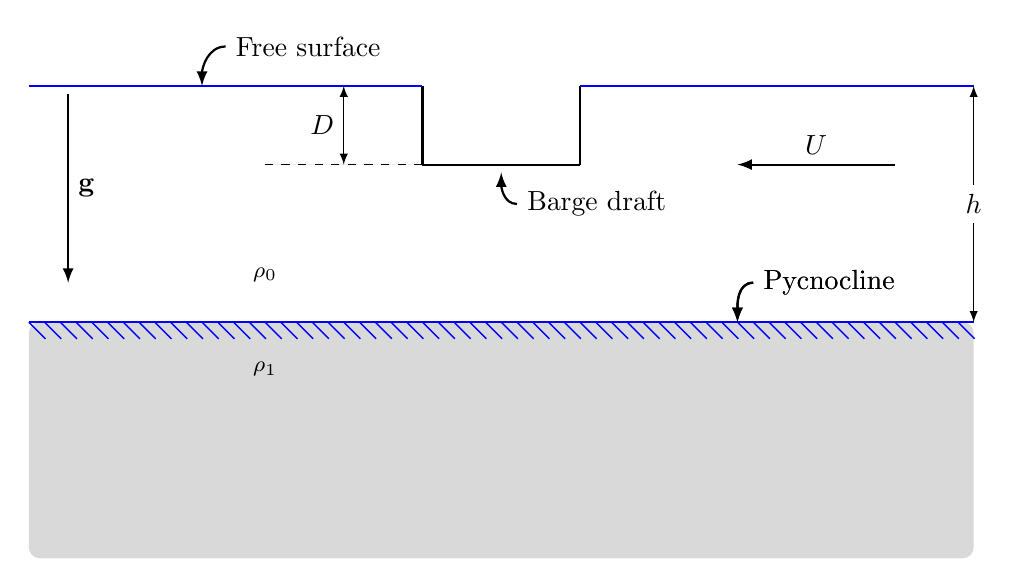
\begin{tikzpicture}[
    media/.style={font={\footnotesize\sffamily}},
    wave/.style={
        decorate,decoration={snake,post length=1.4mm,amplitude=2mm,
        segment length=2mm},thick},
    interface/.style={
        % The border decoration is a path replacing decorator. 
        % For the interface style we want to draw the original path.
        % The postaction option is therefore used to ensure that the
        % border decoration is drawn *after* the original path.
        postaction={draw,decorate,decoration={border,angle=-45,
                    amplitude=0.3cm,segment length=2mm}}},
    dimen/.style={<->,>=latex,thin,
        every rectangle node/.style={fill=white,midway,font=\sffamily}},
    ]
    % Round rectangle
    \fill[gray!30,rounded corners] (-6,-3) rectangle (6,0);
    % Interface
    \draw[blue,line width=.5pt,interface](-6,0)--(6,0);
    % barge
    \draw[thick,black](-1,3)--(-1,2);
    \draw[thick,black](-1,2)--(1,2);
    \draw[thick,black](1,2)--(1,3);
        \draw[-latex,thick](3.2,0.5)node[right]{Pycnocline}
         to[out=180,in=90] (3,0);
    % free surface     
    \draw[thick,blue](-6,3)--(-1,3);
    \draw[thick,blue](1,3)--(6,3);
    % Coordinates system
    %\draw(0,0.15)node[above]{$x$};
    %\draw[<->,line width=1pt] (1,0) node[above]{$y$}-|(0,-1) node[left]{$z$};

    % Media names
    \path[media] (-3,.6)  node {$\rho_0$}
                 (-3,-.6) node {$\rho_1$};
    \draw[dimen] (6,3) -- (6,0) node {$h$};
    \draw [-latex,thick](5,2) -- (3,2)	node [midway,above] {$U$};
    \draw [-latex,thick](-5.5,2.9) -- (-5.5,0.5)	node [midway,right] {$\mathbf{g}$};    
	\draw [fill=gray,dashed] (-1, 2) --(-3, 2); 
	\draw[dimen] (-2,3) -- (-2,2) node [left] {$D$};
    % $x$ axis

    % Interface pointer
    \draw[-latex,thick](3.2,0.5)node[right]{Pycnocline}
         to[out=180,in=90] (3,0);
    % Barge pointer
    \draw[-latex,thick](0.2,1.5)node[right]{Barge draft}
         to[out=180,in=270] (0,1.9);
    % Free surface pointer
    \draw[-latex,thick](-3.5,3.5)node[right]{Free surface}
         to[out=180,in=90] (-3.8,3);         
    % To-paths are really useful for drawing curved lines. The above
    % to path is equal to:
    %
    % \draw[-latex,thick](3.2,0.5)node[right]{$\mathsf{S_{1,2}}$}
    %      ..controls +(180:.2cm) and +(up:0.25cm) .. (3,0);
    % Internally the to path is translated to a similar bezier curve,
    % but the to path syntax hides the complexity from the user. 
\end{tikzpicture}
\caption{Simulation set-up. \\ \textit{Simulations is done by varying speeds $U$ at constant $h/D = 1$, $1.5$ and $2$. Densities $\rho_0$ and $\rho_1$ is that of fresh- and salt-water respectively for stratified fluid simulations. For non-stratified fluid simulations, $\rho_0 = \rho_1$ }}
\label{fig:experiment}
\end{figure}

\section{Boundary and Initial conditions}
Before simulating and solving the numnerical experiment, the momentum and continuity equations (\ref{eqn:momentum} \ref{eqn:continuity}) must have appropriate initial and boundary conditions.\\
\\
Boundary conditions are required component of the mathematical model that directs the motion of the flow. It specifies the fluxes such as mass and momentum into and out of the computational domain.\\
\\
OpenFOAM is representing boundaries as patches consisting of faces, and all inital and and boundary data are assigned to the patches. Table \ref{tbl:boundaries} is showing an overview of all initial and boundary conditions for simulations using the turbulence modell k-omega SST .\\
\\
\begin{landscape}
	\begin{table}[H]
		\centering
		\begin{tabular}{c|c|c|c|c|c|c|c}
			\multicolumn{2}{c|}{\diagbox{Boundary}{Variable}} & U&p$\_$rgh & alpha.saltWater  & k & omega & nut \\\cline{1-8}
			
			\multirow{2}*{Inlet} & Type & fixedValue & fixedFluxPressure & fixedValue &  fixedValue & fixedValue & fixedValue\\
			&Value & internalField & internalField & internalField &  internalField & internalField &internalField \\\cline{1-8}
			
			\multirow{2}*{Outlet} & Type & O.P.M.V. & zeroGradient & V.H.F.R. &  inletOutlet & inletOutlet & zeroGradient\\
			&Value & internalField & - & internalField &  internalField & internalField &- \\\cline{1-8}
			
			\multirow{2}*{Barge} & Type & M.W.V. & F.F.P. & zeroGradient & kqrW.F. & omegaW.F. & nutUSpaldinW.F.\\
			&Value & (0 0 0) & internalField & - & internalField & internalField &internalField \\\cline{1-8}
			
			\multirow{2}*{atmosphere} & Type & slip & fixedValue & zeroGradient & zeroGradient & zeroGradient & zeroGradient\\
			&Value & - & internalField & - &  - &- &-\\\cline{1-8}
			
			\multirow{2}*{atmosphereFrontOfBarge} & Type & inletOutlet & fixedValue & zeroGradient &  zeroGradient & zeroGradient & zeroGradient\\
			&Value & internalField & internalField & - & - & - &-\\\cline{1-8}
			
			\multirow{2}*{Front} & Type & symmetryPlane & symmetryPlane & symmetryPlane &  symmetryPlane &symmetryPlane & symmetryPlane\\
			&Value & - & -& - & - &- &-\\\cline{1-8}
			
			\multirow{2}*{Back} & Type & symmetryPlane & symmetryPlane & symmetryPlane & symmetryPlane & symmetryPlane & symmetryPlane\\
			&Value & - & - & - & - & -& -\\\cline{1-8}
			
			\multirow{2}*{Bottom} & Type & symmetryPlane & symmetryPlane & symmetryPlane &  symmetryPlane & symmetryPlane & symmetryPlane\\
			&Value & - & - & - & - & -& -\\\cline{1-8}
			
		\end{tabular}
		\caption{Boundary and initial conditions twoLiquidMixing with k-omega SST turbulence model.\\
			O.P.M.V. = OutletPhaseMeanVelocity, V.H.F.R. = variableHightFlowRate, M.W.V. = movingWallVelocity, F.F.P. = fixedFluxPressure,\\ kqrW.F. = kqrWallFunction, omegaW.F. = omegaWallFunction, nutUSpaldingW.F. = nutUSpaldingWallFunction}
		\label{tbl:boundaries}
	\end{table}
\end{landscape}

\subsection{U}
For velocity U, typical dirichlet boundary conditions is a applid at the inlet and on the barge. At the inlet there is \textit{fixedValue}  while a no-slip condition is set at the barge. The no-slip condition is a of a special kind, namely \textit{movingWallVelocity}, which is applied for "moving" walls when it is a moving reference frame.\\
\\
At outlet there is an \textit{outletPhaseMeanVelocity}. This boundary condition adjusts the velocity for the given phase to achieve the specified mean, thus causing the phase-fraction to adjust according to the mass flow rate.\\
\\
\subsubsection{Boundary conditions at the free surface}
Since the simulation only includes what happens below the water surface, and the main focus of the experiments is the investigation of the internal wave it, has been rather tricky to decide boundaries for the free surface. The free surface waves that is generated should bee of very small wave length and height due to low Froude numbers (\ref{eqn:FroudeNumber}), as $Fr \leq 0.09 $. An approach has been to apply a Neumann boundary condition of zero gradient at the top. With a zero gradient at the top, the bow of the barge would have been well approximated as the fluid hits the bow and it would allow outflow. At the stern however, the lower pressure would allow inflow. This would have been a good approximation, if the inflow had been consisting of air. The problem is that the inflow at the stern consists of water, causing the interface at the stern to mix and loosing of the stratified water. \\
\\
Another approach as been to use a slip condition, which is a mix of Dirichlet and Neumann condition. The flow would then be allowed to flow freely in x- and y direction, but be set at z-direction. This would not allow for in- and outflow.\\
\\
With the low Froude number and the goal of the invistigation beeing the internal wave, this could have been a good approximation. The \textit{slip} condition caused an numerical artifact at at a point of the bow of the barge where another boundary condition of symmetry was set. The \textit{symmetryPlane} condition at the front of the domain allows outflow, causing a one cell intersecting both boundary conditions having very large velocity.\\
\\
A comprimise has been done, with the top of the domain beeing split into two patches, namely \textit{atmosphere} and \textit{atmosphereFrontOfBarge}. The \textit{atmosphere} patch having a \textit{slip} boundary condition and the \textit{atmosphereFrontOfBarge} having an \textit{inletOutlet} condition. The \textit{inletOutlet} condition is working as a Neumann condition, with the specification of inflow, in case there is any. \\
\\
These boundary conditions has a very engineering approach to them, and is not very physical. But as stated earlier in this repert, the main focus is the effect of the internal wave. With the air excluded completely from the simulations, and the low Froude numbers, the final boundary conditions of the free surface is sufficient with the goal of the experiment.
\subsection{alpha.saltWater}
The phase fraction \textit{alpha.saltWater} is set in the file \textit{setFieldsDict} where the initial state of the fluid is set.\\
\\
As for the boundaries, a fixed value of either $1$ or $0$ is set, where $1$ is salt water and $0$ is fresh water, is set at the inlet. At the outlet, a \textit{variableHightFlowRate} condition is used. It is a phase fraction condition based upon the flow conditions. Values of \textit{alpha.water} is constrained to lay between specified values of upper and lower bounds of $1$ and $0$, i.e.
\begin{itemize}
\item If \textit{alpha.water} > 1:
	\begin{itemize}
	\item apply a fixed value, with a uniform level $1$.
\end{itemize}
\item If $0$ $\leq$ \textit{alpha.saltWater} $\leq$ $1$:
	\begin{itemize}
	\item apply a \textit{zeroGradient} condition.
	\end{itemize}
\item If \textit{alpha.water} < 0:
	\begin{itemize}
	\item apply a fixed value, with a uniform level $0$.
\end{itemize}
\end{itemize}
At the \textit{barge}, a Neumann condition of \textit{zeroGradient} is applied. The same goes for \textit{atmosphere} and \textit{atmosphereFrontOfBarge}.
\subsection{p\_rgh}
For pressure, a \textit{fixedFluxPressure} is used at the inlet and on the barge. The pressure is not known at inlet. The \textit{fixedFluxPressure} is a Neumann condition that is accounting for the flux specified by the velocity set at the boundary.\\
\\
For the barge, the velocity is set to 0 by the \textit{noSlip} boundary condition, so the Neumann  condition becomes a \textit{zeroGradient} in reality.\\
\\
At the athmospere and atmosphereFrontOfBarge patches there is Dirichlet boundary of \textit{fixedValue} 0. At the outlet there is a Neumann boundary condition of \textit{zeroGradient}. 
\subsection{Turbulence properties k, nut, omega and epsilon}
All of the turbulence properties nut, k, omega and epsilon are set with \textit{zeroGradient} at the top patches \textit{atmosphere} and \textit{atmosphereFrontOfBarge}.\\
\\
At the inlet, Dirichlet boundaries are set as a fixed value, calculated from equations for setting farfield turbulence conditions.\\
\\
Farfield turbulent kinetic energy is set by using:
\begin{equation}
k = \frac{3}{2}(UI)^2,
\label{eqn:turbulentKineticEnergy}
\end{equation}
where U is the freestrem speed and I is the turbulence intensity, usually set below 1\% for cases similar to this experiment. \\
\\
Farfield omega conditions is set by using:
\begin{equation}
\omega = \frac{\sqrt{k}}{C_{\mu}^{1/4}l_t}
\label{eqn:turbulentOmega}
\end{equation}
where $C_{\mu}=0.09$ and $l_t$ is the turbulent length scale, set to $l/100$ where l is the length of the barge.\\
\\
Turbulent dissipation rate epsilon is set by using:
\begin{equation}
\epsilon =  \frac{c_{\mu}^{3/4} k^{3/2}}{l_t}
\label{eqn:turbulentDissipationRate}
\end{equation}
Finally, the turbulent viscosity is set by using:
\begin{equation}
\nu_t = \frac{k}{\omega}
\label{eqn:turbulentViscosityFarfield}
\end{equation}
\subsubsection{Wall functions}
Wall funtions are used to avoid resolving all scales in the boundary layer. The wall functions use the dimensional analysis of the boundary layer and law of the wall to estimate values near the wall.\\
\\
At the barge, wall functions are applied as boundary conditions for all the turbulence properties.\\
\\
Turbulent viscosity $\nu_t$ is using the wall function \textit{nutUSpaldingWallFunction}. The function is using a special curve fit of the law of the wall, in order to be applicable in the whole boundary layer \cite{Spalding}.\\
\\
For turbulent kinetic energy $k$, the wall function \textit{kqrWallFunction} has been used. It uses the log-law layer (\ref{eqn:logLayer}) to estimate values for the boundary. Using this wallFunction would require a distance of the first cell adjecent to the barge to be $y^+ > 30$. This has not been fulfilled with the meshes used in this report, but brief test runs with a wall function applicable for smaller values of $y^+$, has been conducted after the mistake was discovered. \textit{kLowReWallFunction} did not make any signifacant effects on the calculated drag in these test runs.\\
\\
For omega and epsilon, the wall functions \textit{omegaWallFunction} and \textit{epsilonWallFunction} has been used. Both wall functions are applicable for a wide range og $y^+$ values.
\section{Mesh and mesh convergence}
The outcome of a numerical experiment is highly dependent on the mesh quality. A multiphase simulation investigating drag and internal waves needs a mesh suitable to capture the phenomenon. At the same time the mesh has to account for computational cost, as the computational resources available is rather limited for the scope of this thesis.
\subsection{Meshing procedure}
The background mesh, or rather the base mesh is made by defining a \textit{blockMeshDict} file that generates a mesh that is refined in the area of the pycnocline shown in figure \ref{fig:baseMesh}. The base mesh is made to be uniform in the spatial x- and y-direction, except for z-direction, where it is refined to better capture the pycnocline in the entire computational domain. Number of cells in the base mesh is 12668. In order to increase mesh quality, refinement is needed.\\
\\
\begin{figure}[H]
	\centering
	\includegraphics[width=0.8\textwidth]{/home/peterek/OpenFOAM/PETER-5.0/MT_PK/plots/paraView/MESH/meshBeforeRefinement.png}
	\caption{Base mesh generated by blockMesh\\ \textit{The base mesh made in blockMeshDict and generated by blockMesh consists of $12668$ cells. It has uniform spatially distribution in x- and y- direction, while z-direction is refined in the area where pycnocline is located.}}
	\label{fig:baseMesh}
\end{figure}

To refine the mesh further, \textit{topoSetDict} and \textit{refineMeshDict} files has been used. In a \textit{topoSetDict}, an area within the mesh is defined which where it is desirable to refine the mesh. The \textit{refineMeshDict} refines the mesh in the specified area in the desired direction. \textit{RefineMeshDict} refines the mesh by splitting every cell within the specified area and in the specified direction.\\
\\
By using \textit{topoSetDict} and \textit{refineMeshDict} it is easy to refine the mesh in the important areas within the domain i.e. boundary layer and below the barge at the pycnocline. It is further a useful tool in the means of maintaining cell aspect ratios, which is the ratio of the longest to the shortest side of the cell. Cell aspect ratio can have significant effect on waves in openFOAM \cite{Roenby}. The areas of the domain which is almost un disturbed can be un-refined, making the mesh less computational demanding.\\
\\
Figure \ref{fig:RefinedMesh} is showing the mesh after refinenemt which consists of $744794$ cells. 
\begin{figure}[H]
	\centering
	\includegraphics[width=0.8\textwidth]{/home/peterek/OpenFOAM/PETER-5.0/MT_PK/plots/paraView/MESH/meshAfterRefinement.png}
	\caption{Mesh after refinement\\ \textit{The mesh after beeing refined consists of $744794$ cells. Max aspect ratio $= 32.7$  }}
	\label{fig:RefinedMesh}
\end{figure}
\subsection{Convergence tests}
Three mesh grids has been systematically refined to evaluate grid convergence. It is done by using a grid refinement ratio of $2$ on the base mesh. The resulting course, medium and fine grids have $4.2\times 10^5$, $7.4\times 10^5$ and $1.3\times 10^6$ cells respectively. The reason for not having a refinement ratio of $2$ on the resulting grids is that the same \textit{topoSetDict} and \textit{refineMeshDict} files are used. The resulting grids does not necessarily get the same refinement ratio, as the refinement procedure using \textit{topoSetDict} and \textit{refineMeshDict} depends on the base mesh.\\
\\
Two speeds at two different pycnocline depths are used to check for convergence, resulting in  four tests. For each pycnocline depth, two velocities gives  densimetric Froude number corresponding to near-peak drag coefficient and densimetric Froude number close to super critical.\\
\\
Figure \ref{fig:convTestIf01U01} and \ref{fig:convTestIf01U022} are showing test runs with pycnocline located at $0.1$m ($h/D = 1$) below the barge and with $Fr_h = 0.86$ and $Fr_h = 1.35$ respectively. Turbulence model used in the tests are the $k-\omega$ SST. The tests show that there is not much difference between the medium and fine grids, while the corse grid is oscillating around a value of $C_d$ i.e. it has not converged.\\
\\
Table \ref{tbl:YplussValuesConvergenceTest1} shows the avarage $y^+$ values obtained from the convergence tests. The $y^+$ values lies all within the buffer layer, suggesting that the Wall functions must be applicable for a wide range of $y^+$ values.
\begin{table}[H]
\centering
\begin{tabular}{c|c|c}
\diagbox{Mesh}{$Fr_h$} & {0.86} & {1.35} \\
\cline{1-3}
\ Coarse	& 11.14	& 13.10 \\\cline{1-3}
\ Medium	&  8.39	& 11.33	\\\cline{1-3}
\ Fine		&  6.8	&  8.95	\\
\end{tabular}
\caption{Average $y^+$ values for pycnocline at $0.1$m  \\ \textit{Average $y^+$ value obtained from running convergence tests.\\ All $y^+$ values lies within the buffer layer, with the finest mesh tending towards viscous sub-layer}}
\label{tbl:YplussValuesConvergenceTest1}
\end{table}

\begin{minipage}{.45\textwidth} 
	\begin{figure}[H]
		\centering
		\includegraphics[width=0.99\textwidth]{/home/peterek/OpenFOAM/PETER-5.0/MT_PK/plots/meshSensitivity/U014Interface01.png}
		\caption{$C_d$ as a function of time. \\ \textit{Grid convergence test run with three different grids; coarse, medium and fine. Pycnocline located at $0.2$ m below the barge, and $Fr_h = 0.61$. The medium and fine grids are converging towards the same drag coefficient, while the coarse grid is occilating around the medium and fine grids}}
		\label{fig:convTestIf01U01}
	\end{figure}
\end{minipage}\hfill
\vspace{2ex}
\begin{minipage}{.45\textwidth} 
	\begin{figure}[H]
		\centering
		\includegraphics[width=0.99\textwidth]{/home/peterek/OpenFOAM/PETER-5.0/MT_PK/plots/meshSensitivity/U022Interface01.png}
		\caption{$C_d$ as a function of time. \\ \textit{Grid convergence test run with three different grids; coarse, medium and fine. Pycnocline located at $0.2$ m below the barge, and $Fr_h = 0.61$. The medium and fine grids are converging towards the same drag coefficient, while the coarse grid is occilating around the medium and fine grids}}
		\label{fig:convTestIf01U022}
	\end{figure}
\end{minipage}\hfill
\vspace{2ex}\\
\\
Figure \ref{fig:convTestIf02U016} and \ref{fig:convTestIf02U022} are showing test runs with pycnocline located at $0.2$m ($h/D=2$) below the barge and with $Fr_h = 0.61$ and $Fr_h = 0.95$ respectively. Turbulence model used in the tests are the $k-\omega$ SST. The tests show the same trends as the tests done with pycnocline located $0.1$m below the barge.\\
\\
Table \ref{tbl:YplussValuesConvergenceTest2} shows the avarage $y^+$ values obtained from the convergence tests with pycnocline located at $0.2$m below the barge. The $y^+$ values lies all within the buffer layer, suggesting that the Wall functions must estimate the whole turbulent boundary region
\begin{table}[H]
\centering
\begin{tabular}{c|c|c}
\diagbox{Mesh}{$Fr_h$} & {0.61} & {0.95} \\
\cline{1-3}
\ Coarse	& 11.89	& 14.50 \\\cline{1-3}
\ Medium	&  9.74	& 11.53	\\\cline{1-3}
\ Fine		&  7.73	& 9.51	\\
\end{tabular}
\caption{Average $y^+$ values for pycnocline at $0.2$m  \\ \textit{Average $Y^+$ value obtained from running convergence tests.\\ All $Y^+$ values lies within the buffer layer, with the finest mesh tending towards viscous sub-layer}}
\label{tbl:YplussValuesConvergenceTest2}
\end{table}
\begin{minipage}{.45\textwidth} 
	\begin{figure}[H]
		\centering
		\includegraphics[width=0.99\textwidth]{/home/peterek/OpenFOAM/PETER-5.0/MT_PK/plots/meshSensitivity/U014Interface02.png}
		\caption{$C_d$ as a function of time. \\ \textit{Grid convergence test run with three different grids; coarse, medium and fine. Pycnocline located at $0.2$ m below the barge, and $Fr_h = 0.61$. The medium and fine grids are converging towards the same drag coefficient, while the coarse grid is occilating around the medium and fine grids}}
		\label{fig:convTestIf02U016}
	\end{figure}
\end{minipage}\hfill
\vspace{2ex}
\begin{minipage}{.45\textwidth} 
	\begin{figure}[H]
		\centering
		\includegraphics[width=0.99\textwidth]{/home/peterek/OpenFOAM/PETER-5.0/MT_PK/plots/meshSensitivity/U022Interface02.png}
		\caption{$C_d$ as a function of time. \\ \textit{Grid convergence test run with three different grids; coarse, medium and fine. Pycnocline located at $0.2$ m below the barge, and $Fr_h = 0.61$. The medium and fine grids are converging towards the same drag coefficient, while the coarse grid is occilating around the medium and fine grids}}
		\label{fig:convTestIf02U022}
	\end{figure}
\end{minipage}\hfill
\vspace{2ex}
\\
\\
From the convergence tests it is clear that it is not much to gain convergence wise by using a finer mesh. The resulting $C_d$'s are very similar comparing the medium and fine grids. By using the medium mesh, computational time is saved and many more simulations  can be done within the time frame of this thesis.   

\chapter{Results}
\section{Comparison of turbulence models}
Comparison of the turbulence models was done by running numerical experiments with the exact same mesh. The tests was done with a pycnocline depth of $0.2$m below the barge. Two cases are presented, the first with a densimetric Froude number $Fr_h=0.69$ and the second with $Fr_h=0.95$. The first test lies whithin the range where $Fr_h$ should give peak $C_d$ and the second test where $Fr_h$ should give a lower $C_d$ that tends towards a non-stratified fluid case.\\
\\
The comparison is done by checking convergence of the $C_d$ for the two cases. The motivation for comparing the $C_d$ and not any other parameters is that of the main scope of this project, investigating the increase in $C_d$ in the range of $0.6\leq Fr_h \leq 0.8$ in stratified fluids. It is essential to have a turbulence model that best approximate the $C_d$ \\
\\
The first test is shown in figure \ref{fig:turbulenceModelComparison1}. From the figure it is shown that the turbulence model $k-\omega$ SST gives a good convergence of the $C_d$. The model $k-\epsilon$ on the other hand sees an increace of $C_d$ throughout the entire expriment and gets even more unstable as time increases.\\
\\
THe second test is shown in figure \ref{fig:turbulenceModelComparison2}, and is showing the same trend as seen in the first test. $k-\omega$ SST gives a good convergence, while $k-\epsilon$ gets an increase in $C_d$ as time increases. In the second test, $k-\epsilon$ even starts to oscillate as the time increases.\\
\\
From the tests it is concluded that $k-\omega$ SST model is the most reliable investigating the "dead water" phenomenon going further.\\
\\
Even though the theory states that the $k-\omega$ turbulence model yields better results when simulating adverse pressure gradients and boundary layer \cite{CFD}, it serves a purpose to compare with other models. As stated in theory, the $k-\epsilon$ model can get reliable results when simulating multiphase fluids. The comparison of the models only confirms the theory that the $k-\omega$ SST model is superior in estimating boundary layers and adverse pressure gradients.\\
\\
\begin{minipage}[t]{.45\textwidth}
	\begin{figure}[H]
		\centering
		\includegraphics[width=0.99\textwidth]{/home/peterek/OpenFOAM/PETER-5.0/MT_PK/plots/turbulenceModelComparison/U016.png}
		\caption{$C_d$ as a function of time.\\ \textit{Simulations done with a pycnocline at $0.2$m and $Fr_h=0.69$. $k-\epsilon$ Turbulence model yields a higher $C_d$ than the $k-\omega$ SST model. While the $k-\omega$ SST model converges, $k-\epsilon$ model has a steady growth of $C_d$ and gets more unstable as time increases}}
		\label{fig:turbulenceModelComparison1}
	\end{figure}
\end{minipage}\hfill
\vspace{2ex}
\begin{minipage}[t]{.45\textwidth} 
	\begin{figure}[H]
		\centering
		\includegraphics[width=0.99\textwidth]{/home/peterek/OpenFOAM/PETER-5.0/MT_PK/plots/turbulenceModelComparison/U022.png}
		\caption{$C_d$ as a function of time.  \\ \textit{Simulations done with a pycnocline at $0.2$m and $Fr_h=0.95$. $k-\epsilon$ Turbulence model yields a higher $C_d$ than the $k-\omega$ SST model. While the $k-\omega$ SST model converges, $k-\epsilon$ model has a steady growth of $C_d$ and starts to oscillate as time increases}}
		\label{fig:turbulenceModelComparison2}
	\end{figure}
\end{minipage}\hfill
%\vspace{2ex}

\section{Drag}
\subsection{Non-stratified fluid}
Non-stratified fluid simulations was conducted by simulating with a density corresponding to fresh water and with barge draft $D=0.1$m at speeds $0.06$m$s^{-1}$ $\leq$ $U$ $\leq$ $0.24$m$s^{-1}$. \\
\\
Gou et.al conducted the same experiment in a towing tank, with the same dimensions on the barge. Their results showed that drag force is directly proportianal to the square of the towing speed, which means that the $C_d$ is constant.\\
\\
In figure \ref{fig:dragForce} results of the non-stratified fluid simulations is shown along with the results obtained by Gou et.al. \cite{Gou}. The figure is showing drag force as function of the velocity squared. Similar to the results by Gou et. al, this paper is getting a linear curve, meaning the non-stratified flow has a constant $C_d$ for all speeds.\\
\\
The current study underpredicts the drag force obtained by Gou et.al. by $\approx 20\%$. There may be sevaral reasons for the under-prediction of drag. Reason one beeing that the Gou et.al study did experiments in a shallow water tank, while this simulation domain is much larger. Another reason is the approach of not including what is above water line and excluding the free surface.\\
\\
\begin{figure}[H]
	\centering
	\includegraphics[width=0.75\textwidth]{/home/peterek/OpenFOAM/PETER-5.0/MT_PK/plots/3Dtop/Gou2KOSpaldingRefType2kLowRe.png}
	\caption{Drag force as function of velocity squared. \\ \textit{Resistance in homogeneous fluid with barge draft $=0.1$. Simulations is in good agreement with experimental data obtained on an identical barge done by Gou et. al. \cite{Gou} with a deviance of $\approx 20$ \%. Drag force is directly proportianal to the square of the towing speed, which means that the $C_d$ is constant. }}
	\label{fig:dragForce}
\end{figure}
\subsection{Stratified fluids}
Study of the behaviour of $C_d$ in a stratified fluid is conducted by simulating with barge draft $D=0.1$ and pycnocline depths $h/D=1$, $1.5$ and $2$. All three set ups are then simulated with speeds corresponding to densimetric Froude numbers (\ref{eqn:densimetricFroudeNumber}) in the range of $0.35\leq Fr_h \leq 1.35$\\
\\
The $C_d$ shown in figure \ref{fig:Cd} offers a lot of information. A clear pattern of increasing $C_d$ is shown for all three pycnocline depths. All $C_d$ peaks are found within the range of $0.6 \leq Fr_h \leq 0.7$, with pycnocline depth $h/D=1$ giving the largest $C_d$. All three set-ups are giving the same pattern in $C_d$ of increasing as $Fr_h$ approaches peak $C_d$ and then decrasing again and tending towards non-stratified fluids.\\
\\
Similar trends are presented in the study done by Esmaeilpour et. al. \cite{Esmaeilpour} who are doing computational fluid dynamics study on a vessel sailing in stratified waters.  Esmaeilpour et. al. had peaks between $Fr_h=0.83$ and $Fr_h=0.91$, which is in a range a bit higher than peaks presented in this study.\\
\\
Esmaeilpour et.al. is also reporting a much more significant increase in $C_d$ than is obtained in this report. The peak $C_d$ for a pycnocline depth of $h/D=1$ has an increace of $600\%$.
\begin{figure}[H]
	\centering
	\includegraphics[width=0.75\textwidth]{/home/peterek/OpenFOAM/PETER-5.0/MT_PK/plots/3Dtop/esmaeilpourSpaldingRefType2kLowRe.png}
	\caption{Drag coefficient as function of $Fr_h$  \\ \textit{Drag coefficients ($C_d$) obtained by running simulations with pycnocline depth $h/D=1$, $1.5$ and $2$. $C_d$ peaks within a range of $Fr_h = 0.6$ and $0.8$. $C_d$ tends towards simulations of non-stratified fluid for all pycnocline locations when $Fr_h \leq 0.6$ and $Fr_h \geq 0.8$.}}
	\label{fig:Cd}
\end{figure}
Percentage increace of $C_d$ is presented in figure \ref{fig:CdPercentageDifference}, and it show that for pycnocline depth $h/D=1$ has a percentage increase of $21\%$. Looking at $h/D=1.5$ there is an increase of $13.5\%$, while Esmaeilpour et.al has an increase of $450\%$ for the same pycnocline.\\
\\
Looking into the large difference in the increase of $C_d$, the question arises of the exclusion of the free-surface. The effects of the free-surface might be to significant in stratified waters to leave out the free surface. Another key difference in the approach done by Esmaeilpour et.al. is the number of grids. The study was conducted with a grid consisting of $21.9\times 10^6$ cells, to properly resolve boundary layer and internal wave appearing at the pycnocline.\\
\\
Despite of the small amount of increase in $C_d$ obtained from the simulations, the effect of the stratified fluid is clearly apparent. The increase in drag appears in the same manner presented in Gou et.al. \cite{Gou}. It is also in accordance with the findings in the study of FRAM's dead water resistance conducted by Grue \cite{Grue}. Grue 
\begin{figure}[H]
	\centering
	\includegraphics[width=0.75\textwidth]{/home/peterek/OpenFOAM/PETER-5.0/MT_PK/plots/3Dtop/esmaeilpourSpaldingRefType2kLowRePercentage.png}
	\caption{Percentage increase as function $Fr_h$.  \\ \textit{Percentage difference between stratified and non stratified fliuds. Pycnocline depth of  $h/D=2$ gives a peak difference of $8.5\%$. $h/D=15$m gives peak difference of $13.5\%$ and $h/D=1$ gives peak difference of $21\%$}}
	\label{fig:CdPercentageDifference}
\end{figure}
\section{Internal wave and its effect}
Any kind of vessel propagating in stratified fluids experience increase in drag compared to non-stratified fluid. As the barge propagates in the stratified fluid, internal waves appear below the barge. The numerical experiments is cathing this phenomeneon, and it is clearly an internal wave below the barge.\\
\\
\subsection{Vizualization of the internal wave}
Figure \ref{fig:velocityAndPycnoclineIf02U016Test} is a visualization of the internal wave below the barge. It is showing a contour of the $\alpha$ fraction for a pycnocline depth $h/D=2$, and a non dimensionalized x-direction velocity located at the symmetry plane. The figure is showing a wave pattern, but the figure is only giving empirical evidence of the internal wave. The figure is a useful tool for visualizing the phenomenon. 
\begin{figure}[H]
	\centering
	\includegraphics[width=0.75\textwidth]{/home/peterek/OpenFOAM/PETER-5.0/MT_PK/plots/paraView/velocityAndNormalsZ/VelocityAndPycnoclineNormalsZIf02U016Test.png}
	\caption{Contour of $\alpha$ below the barge \\ \textit{Contour of the value fraction $\alpha$ at the pycnocline depth $h/D=2$. An internal wave appears below the barge. The non dimensional velocity $U_x/U_{0x}$ is shown in the symmetryplane of the domain.}}
	\label{fig:velocityAndPycnoclineIf02U016Test}
\end{figure}
\subsection{Wave location and effect on velocity}
The densimetric Froude number (\ref{eqn:densimetricFroudeNumber}) is a ratio of the velocity of the barge and the celerity of the longest internal waves. As $Fr_h$ increases, the largest crest of the internal wave is going to be located at further and furter back towards the stern of the barge, and eventually be behind it.\\
\\
Figure \ref{fig:eta1} is showing the location of the pycnocline as a function of it position below the barge. The three cases shown in the figure corresponds to $Fr_h$ where $C_d$ starts to increase, $Fr_h$ at peak $C_d$ and $Fr_h$ where $C_d$ has decreased and almost reached a $C_d$ obtained by non-stratified simulations.\\
\\
The location of the internal wave corresponding to peak $C_d$ is located in the wake and almost right below the stern of the barge. The internal waves are causing restriction of passage area, and the flow is accelerated. Acceleration of the fluid flow is thinning the boundary layer and causing a drop in pressure.\\
\\
Figure \ref{fig:velocityProfileX0}, is showing non-dimensional velocity profiles scaled by the far field velocity. The velocity profile corresponding to the internal wave located below the stern of the barge shows increase in velocity as it approches the stern. This in turn makes the pressure dop and a thinning of the boundary layer, causing an increase in $C_d$.\\
\\Pycnocline depth $h/D=1.5$ is telling the same story as for pycnocline depth $h/D=2$. Looking at figure \ref{fig:eta2} and figure \ref{fig:velocityProfileX0If15}, the internal wave located below the stern of the barge corresponding to peak $C_d$ is causing the increace in velocity\\
\\
\begin{minipage}[t]{.45\textwidth} 
	\begin{figure}[H]
		\centering
		\includegraphics[width=0.99\textwidth]{/home/peterek/OpenFOAM/PETER-5.0/MT_PK/plots/3Dtop/Surface.png}
		\caption{Pycnocline as a function of x-position. \\ \textit{Initial pycnocline depth $h/D=2$. As $Fr_h$ increases, wave amplitude increase and the crest located further back. Location of crest has significant effect on flow field as shown in figure \ref{fig:velocityProfileX0}. The internal wave restricts the passage area, causing a significant increase in speed. This effects on $C_d$ are shown in figure \ref{fig:Cd}.}}
		\label{fig:eta1}
	\end{figure}
\end{minipage}\hfill
\vspace{2ex}
\begin{minipage}[t]{.45\textwidth}
	\begin{figure}[H]
		\centering
		\includegraphics[width=0.99\textwidth]{/home/peterek/OpenFOAM/PETER-5.0/MT_PK/plots/3Dtop/VelocityProfileX0.png}
		\caption{velocity profiles $U_x/U_0$ as function of z-position. \\ \textit{Dimensionlesss velocity profiles $U_x/U_0$ below barge at $x = 0.0$m with pycnocline at $0.2$m. The velocity profile with $Fr_h = 0.69$ has a signifiant increase in speed and greater gradient.}}
		\label{fig:velocityProfileX0}
	\end{figure}
\end{minipage}\hfill
\vspace{2ex}
\begin{minipage}[t]{.45\textwidth} 
	\begin{figure}[H]
		\centering
		\includegraphics[width=0.99\textwidth]{/home/peterek/OpenFOAM/PETER-5.0/MT_PK/plots/3Dtop/Surface15.png}
		\caption{Pycnocline as a function of x-position. \\ \textit{Initial pycnocline depth $h/D=2$. As $Fr_h$ increases, wave amplitude increase and the crest located further back. Location of crest has significant effect on flow field as shown in figure \ref{fig:velocityProfileX0If15}. The internal wave restricts the passage area, causing a significant increase in speed. This effects on $C_d$ are shown in figure \ref{fig:Cd}.}}
		\label{fig:eta2}
	\end{figure}
\end{minipage}\hfill
\vspace{2ex}
\begin{minipage}[t]{.45\textwidth}
	\begin{figure}[H]
		\centering
		\includegraphics[width=0.99\textwidth]{/home/peterek/OpenFOAM/PETER-5.0/MT_PK/plots/3Dtop/VelocityProfileX0IF15.png}
		\caption{velocity profiles $U_x/U_0$ as function of z-position. \\ \textit{Dimensionlesss velocity profiles $U_x/U_0$ below barge at $x = 0.0$m with pycnocline at $0.2$m. The velocity profile with $Fr_h = 0.69$ has a signifiant increase in speed and greater gradient.}}
		\label{fig:velocityProfileX0If15}
	\end{figure}
\end{minipage}\hfill
\vspace{2ex}\\
\\
Looking at velocity profiles midships at $x=0.30$m in figur \ref{fig:velocityProfileX2If15} and \ref{fig:velocityProfileX2If15}, it is clearly an acceleration of the flow caused by the wave also located midships. Since the wave is located midships, it is not effecting $C_d$ as much as the one located at the stern. A pressure drop midship below the barge is not as significant as one located at the stern.
\\
\\
\begin{minipage}[t]{.45\textwidth} 
	\begin{figure}[H]
		\centering
		\includegraphics[width=0.99\textwidth]{/home/peterek/OpenFOAM/PETER-5.0/MT_PK/plots/3Dtop/VelocityProfileX2.png}
		\caption{velocity profiles $U_x/U_0$ as function of z-position. \\ \textit{Dimensionlesss velocity profiles $U_x/U_0$ below barge at $x = 0.3$m with pycnocline at $0.2$m. The velocity profile with $Fr_h = 0.35$ has a signifiant increase in speed and greater gradient, as the amplitude of the internal wave is located near the same location.}}
		\label{fig:velocityProfileX2If2}
	\end{figure}
\end{minipage}\hfill
\vspace{2ex}
\begin{minipage}[t]{.45\textwidth}
	\begin{figure}[H]
		\centering
		\includegraphics[width=0.99\textwidth]{/home/peterek/OpenFOAM/PETER-5.0/MT_PK/plots/3Dtop/VelocityProfileX2IF15.png}
		\caption{velocity profiles $U_x/U_0$ as function of z-position. \\ \textit{Dimensionlesss velocity profiles $U_x/U_0$ below barge at $x = 0.3$m with pycnocline at $0.15$m. The velocity profile with $Fr_h = 0.40$ has a signifiant increase in speed and greater gradient, as the amplitude of the internal wave is located near the same location.}}
		\label{fig:velocityProfileX2If15}
	\end{figure}
\end{minipage}\hfill
\vspace{2ex}

\chapter{Conclusions and further recommendations}
\section{Conclusions}
Computational fluid dynamics have been used to investigate drag resistance on a barge in stratified and non-stratified waters. The free open source software OpenFOAM has been used to get a qualitative understanding of the dead water phenomenon.\\
\\
A comparison of the RANS turbulence models $k-\epsilon$ and $k-\omega$ SST has been conducted to determine which model is most applicable for the investigation. The comparison consists of convergence tests of the drag coefficients $C_d$ on the barge with draft $D=0.1$m and a pycnocline depth $h/D=2$. $k-\omega$ SST model was suspected to give the best results, which was shown. The $k-\omega$ SST model converged and gave stable results. The $k-\epsilon$ model was found to be unstable, not converging and even oscillating for simulations with densimetric Froude number $Fr_h= 0.95$.\\
\\
Simulations of a non-stratified fluid showed similar behaviour as obtained by Gou et al. \cite{Gou}. The non stratified fluid simulations were shown to have a constant $C_d$, and to have a drag force directly proportional to the square of the simulation speed. Simulations yielded rusults with a deviance of $\approx 20\%$ compared to results from gou et al.\\
\\
Simulations of stratified fluid mostly agree with results obtained by Gou et al \cite{Gou}, J. Grue \cite{Grue} and Esmaeilpour \cite{Esmaeilpour}.  Increase in $C_d$ is shown in all simulations with densimetric Froude number in regions of $0.35 \leq Fr_h \leq 0.6$. Peak $C_d$ was found in regions $0.6 \leq Fr_h \leq 0.7$ and decrease for $fr_h > 0.7$ with $C_d$ tending towards non-stratified simulations as $Fr_h$ increased. The same trend was shown for all pycnocline depths $h/D=1$, $1.5$ and $2$. Gou et al. reported peak in regions $0.5 \leq Fr_h \leq 0.6$, while Esmaeilour et al. reported peaks in regions $0.83\leq Fr_h \leq 0.93$.\\
\\
The increase in drag of stratified fluid was found to be much smaller than reported by Gou et at. and Esmaeilpour et al., with a maximum increase of $21\%$ in $C_d$ compared to a non-stratified fluid. Esmaeilpour reported a maximum increase in $C_d$ of $600\%$. Even though their study was conducted on a completely different vessel, their reported increase is suggesting under-estimation in this report. The reason for the under-estimation of $C_d$ may be the exclusion of the free surface. It is also likely to be due to insufficient number of grid points. Esmaeilpour had around $20$ times more grid points compared to this study, with around $20$ million cells.\\
\\
The internal gravity waves and their location below the barge were found to have significant effect on the flow field. The speed is accelerated by the restriction of passage area by the internal wave. The waves corresponding to the peak $C_d$ caused a significant increase in the velocity at the stern, causing a drop of pressure. \\
\\
\section{Further recommendations}
Further recommendations regarding investigations on the dead water phenomenon, a lot of improvements and approaches can be advised.\\
\\
As this project only focused on the internal wave, and leaving out the free surface waves, it would be of great interest to include the free surface waves in the investigation. A better resolved mesh is advised, especially around the pycnocline. Simulations with pycnocline depths $h/D\leq 1$ should be studied to see for which pycnocline depth a maximum resistance is obtained, and for which depth the effect decreases again.\\
\\
Comparison of other turbulence models e.g. Spalart-Allmaras model is advised, as it is said to have good preformance for flows with adverse pressure gradients and boundary layers \cite{CFD}. A study of sensitivity to numerical discretization schemes may be conducted, in order to obtain higher order of accuracy and stability. Also conducting a comparison of large eddy simulations with RANS simulations is of interest.\\
\\
Experiments in a towing tank, allowing for measuring of resistance in combinations with tools to investigate velocity profiles such as particle mage velocimetry (PIV) should be conducted. A combination of both experiments and CFD could lead to an even better qualitative understanding of the phenomenon. 
\begin{thebibliography}{9}
	\bibitem{Nansen}
	F. Nansen\\
	Farthest North, Westminster: Archibald Constable and Company\\
	2 Whitehall Gardens, 1897. Vol 1.
	
	\bibitem{Ekman}
	V.W. Ekman\\
	On dead-water in The Norwegian North Polar Expidition 1893-1896. Scientific Results.\\
	Edited by F. Nansen (Brogger, christiania, 1904)	
	
	\bibitem{Gou} 
	Y. Guo, W. Xu, X. Xinwei, and B. Teng,\\
	Experiment study on the towing resistance of a barge in a
two-layer fluid.\\
	In The 32nd International Workshop on Water Waves and Floating Bodies, 2017.
	
	\bibitem{Esmaeilpour} 
	Mehdi Esmaeilpour, J. Ezequiel Martin, Pablo M. Carrica\\
	Computational Fluid Dynamics Study of the Dead Water Problem\\
	Journal of Fluids Engineering, October, 2017.
	
	\bibitem{Grue}
	John Grue\\
	calculating FRAM's dead water\\
	Springer Verlag, 2018
	
	\bibitem{AppliedMathematicalModelling} 
	C.D. Argyropoulos, N.C. Markatos, (2015).
	Recent advances on the numerical modelling of turbulent flows, Applied Mathematical Modelling \\
	\url{https://www.sciencedirect.com/science/article/pii/S0307904X14003448#bi0005}

	\bibitem{White} 
	F.M. White,
	Viscous Fluid FLow \\
	(second ed.), McGraw Hill, New York (1991)
	
	\bibitem{reviewOfSSTModel}
	 F. R. Menter \\ Review of the shear-stress transport turbulence model experience from an industrial perspective,\\
	International Journal of Computational Fluid Dynamics (2009)\\
	\url{https://www.tandfonline.com/doi/full/10.1080/10618560902773387?scroll=top&needAccess=true#_i3}
	
	\bibitem{NASA_SST}
	Turbulence Modeling Resource \\
	\url{https://turbmodels.larc.nasa.gov/sst.html}

	\bibitem{Turbulence} 
	Frans T.M. Nieuwstadt, Bendiks J. Boersma, Jerry Westerweel,
	Turbulence, Introduction to Theory and Applications
of Turbulent Flows \\
	 Springer, Delft (2015)
	 
	\bibitem{LESTurbulence} 
     L. C. Berselli T. Iliescu W. J. Layton\\	 
	 Mathematics of Large Eddy Simulation of Turbulent Flows \\
	 Springer, Pisa, Blacksburgh and Pittsburgh (2005)	 
	 
	\bibitem{CFD} 
	H. K. Versteeg, W. Malalasekera, An introduction to Computational Fluid Dynamics, The Finite Volume method\\
	 ( second edition) , Pearson, Loughborough (2007)
	 
	\bibitem{Wilcox} 
	 D. Wilcox\\
	 Turbulence Modelling for CFD\\
	(third ed.), DCW Industries, Inc (2006)
	
	\bibitem{Pope}
	S. P. Pope.\\
	Turbulent Flows.\\
	Cambridge University Press, 2000.

	\bibitem{UNIK4900} 
	 P. Durbin, B. A. Petterson Reif\\
	 Statistical Theory and Modeling for Turbulent Flows\\
	(second ed.), Wiley \& Sons, West Sussex (2011)
	
	\bibitem{VOF1} 
	By Kai Bao, Xiaolong Wu, Hui Zhang and Enhua Wu\\
	Volume fraction based miscible and immiscible fluid animation\\
	Comp. Anim. Virtual Worlds (2010)
	\url{http://citeseerx.ist.psu.edu/viewdoc/download?doi=10.1.1.459.7375&rep=rep1&type=pdf}
	
	\bibitem{VOF2} 
	Gregor Černe, Stojan Petelin † and Iztok Tiselj\\
	Coupling of the Interface Tracking and the Two-Fluid Models 		for the Simulation of Incompressible Two-Phase Flow\\
	Journal of Computational Physics 171, 776–804 (2001)
	\url{https://ac.els-cdn.com/S002199910196810X/1-s2.0-S002199910196810X-main.pdf?_tid=30dd869d-b73f-4eed-ab23-6157367259eb&acdnat=1523609023_364c3bac9fcaf02d04d3586a5b9a78c4}
	
	\bibitem{ITTC}
	International Towing Tank Conference,\\
	Recommended Procedures and Guidelines, Practical Guidelines for Ship CFD Applications
	\url{https://ittc.info/media/1357/75-03-02-03.pdf}
	
	\bibitem{CFDOpenFOAM}
	Fadl Moukalled, Marwan Darwish, and Luca Mangani.\\
	The Finite Volume Method in Computational Fluid Dynamics An Advanced Introduction with 	Open-FOAM(R) and Matlab\\
	volume 113 of Fluid Mechanics and its applications. Springer-Verlag, 2015.
	
	\bibitem{Spalding}
	D. B. Spalding,\\
	A Single Formula for the "Law of the Wall",\\ 
	Journal of Applied Mechanics, (1961).
	
	\bibitem{Krpan}
	Rok Krpan and Boštjan Končar\\
	Simulation of Turbulent Wake at Mixing of Two Confined Horizontal Flows
	Science and Technology of Nuclear Installations,Volume 2018 "Jožef Stefan" Institute, 		Ljubljana, Slovenia
	\url{https://www.hindawi.com/journals/stni/2018/5240361/}\\
	
	\bibitem{SST}	
	Menter, F. R.\\
	Two-Equation Eddy-Viscosity Turbulence Models for Engineering Applications\\
	AIAA Journal, Vol. 32, No. 8, August 1994, pp. 1598-1605.
	
	\bibitem{Roenby}	
	Johan Roenby, Bjarke Eltard Larsen, Henrik Bredmose and Hrvoje Jasak\\
	A new volume of fluid method in OpenFOAM\\
	VII International Conference on Computational Methods in Marine Engineering,MARINE 			2017
	
\end{thebibliography}

\end{document}